% Options for packages loaded elsewhere
\PassOptionsToPackage{unicode}{hyperref}
\PassOptionsToPackage{hyphens}{url}
\PassOptionsToPackage{dvipsnames,svgnames,x11names}{xcolor}
%
\documentclass[
  super,
  preprint,
  3p]{elsarticle}

\usepackage{amsmath,amssymb}
\usepackage{iftex}
\ifPDFTeX
  \usepackage[T1]{fontenc}
  \usepackage[utf8]{inputenc}
  \usepackage{textcomp} % provide euro and other symbols
\else % if luatex or xetex
  \usepackage{unicode-math}
  \defaultfontfeatures{Scale=MatchLowercase}
  \defaultfontfeatures[\rmfamily]{Ligatures=TeX,Scale=1}
\fi
\usepackage{lmodern}
\ifPDFTeX\else  
    % xetex/luatex font selection
\fi
% Use upquote if available, for straight quotes in verbatim environments
\IfFileExists{upquote.sty}{\usepackage{upquote}}{}
\IfFileExists{microtype.sty}{% use microtype if available
  \usepackage[]{microtype}
  \UseMicrotypeSet[protrusion]{basicmath} % disable protrusion for tt fonts
}{}
\makeatletter
\@ifundefined{KOMAClassName}{% if non-KOMA class
  \IfFileExists{parskip.sty}{%
    \usepackage{parskip}
  }{% else
    \setlength{\parindent}{0pt}
    \setlength{\parskip}{6pt plus 2pt minus 1pt}}
}{% if KOMA class
  \KOMAoptions{parskip=half}}
\makeatother
\usepackage{xcolor}
\setlength{\emergencystretch}{3em} % prevent overfull lines
\setcounter{secnumdepth}{5}
% Make \paragraph and \subparagraph free-standing
\ifx\paragraph\undefined\else
  \let\oldparagraph\paragraph
  \renewcommand{\paragraph}[1]{\oldparagraph{#1}\mbox{}}
\fi
\ifx\subparagraph\undefined\else
  \let\oldsubparagraph\subparagraph
  \renewcommand{\subparagraph}[1]{\oldsubparagraph{#1}\mbox{}}
\fi


\providecommand{\tightlist}{%
  \setlength{\itemsep}{0pt}\setlength{\parskip}{0pt}}\usepackage{longtable,booktabs,array}
\usepackage{calc} % for calculating minipage widths
% Correct order of tables after \paragraph or \subparagraph
\usepackage{etoolbox}
\makeatletter
\patchcmd\longtable{\par}{\if@noskipsec\mbox{}\fi\par}{}{}
\makeatother
% Allow footnotes in longtable head/foot
\IfFileExists{footnotehyper.sty}{\usepackage{footnotehyper}}{\usepackage{footnote}}
\makesavenoteenv{longtable}
\usepackage{graphicx}
\makeatletter
\def\maxwidth{\ifdim\Gin@nat@width>\linewidth\linewidth\else\Gin@nat@width\fi}
\def\maxheight{\ifdim\Gin@nat@height>\textheight\textheight\else\Gin@nat@height\fi}
\makeatother
% Scale images if necessary, so that they will not overflow the page
% margins by default, and it is still possible to overwrite the defaults
% using explicit options in \includegraphics[width, height, ...]{}
\setkeys{Gin}{width=\maxwidth,height=\maxheight,keepaspectratio}
% Set default figure placement to htbp
\makeatletter
\def\fps@figure{htbp}
\makeatother

\makeatletter
\makeatother
\makeatletter
\makeatother
\makeatletter
\@ifpackageloaded{caption}{}{\usepackage{caption}}
\AtBeginDocument{%
\ifdefined\contentsname
  \renewcommand*\contentsname{Table of contents}
\else
  \newcommand\contentsname{Table of contents}
\fi
\ifdefined\listfigurename
  \renewcommand*\listfigurename{List of Figures}
\else
  \newcommand\listfigurename{List of Figures}
\fi
\ifdefined\listtablename
  \renewcommand*\listtablename{List of Tables}
\else
  \newcommand\listtablename{List of Tables}
\fi
\ifdefined\figurename
  \renewcommand*\figurename{Figure}
\else
  \newcommand\figurename{Figure}
\fi
\ifdefined\tablename
  \renewcommand*\tablename{Table}
\else
  \newcommand\tablename{Table}
\fi
}
\@ifpackageloaded{float}{}{\usepackage{float}}
\floatstyle{ruled}
\@ifundefined{c@chapter}{\newfloat{codelisting}{h}{lop}}{\newfloat{codelisting}{h}{lop}[chapter]}
\floatname{codelisting}{Listing}
\newcommand*\listoflistings{\listof{codelisting}{List of Listings}}
\makeatother
\makeatletter
\@ifpackageloaded{caption}{}{\usepackage{caption}}
\@ifpackageloaded{subcaption}{}{\usepackage{subcaption}}
\makeatother
\makeatletter
\@ifpackageloaded{tcolorbox}{}{\usepackage[skins,breakable]{tcolorbox}}
\makeatother
\makeatletter
\@ifundefined{shadecolor}{\definecolor{shadecolor}{rgb}{.97, .97, .97}}
\makeatother
\makeatletter
\makeatother
\makeatletter
\makeatother
\journal{Journal of Transport Geography}
\ifLuaTeX
  \usepackage{selnolig}  % disable illegal ligatures
\fi
\usepackage[]{natbib}
\bibliographystyle{elsarticle-num}
\IfFileExists{bookmark.sty}{\usepackage{bookmark}}{\usepackage{hyperref}}
\IfFileExists{xurl.sty}{\usepackage{xurl}}{} % add URL line breaks if available
\urlstyle{same} % disable monospaced font for URLs
\hypersetup{
  pdftitle={Toward Gender-Mainstreaming Transport Planning: Measuring Multimodal Access to Care},
  pdfauthor={Anastasia Soukhov; Léa Ravensbergen; Nicholas Mooney},
  pdfkeywords={Accessibility, Mobility of Care, Gender, Equity, Travel
Mode},
  colorlinks=true,
  linkcolor={blue},
  filecolor={Maroon},
  citecolor={Blue},
  urlcolor={Blue},
  pdfcreator={LaTeX via pandoc}}

\setlength{\parindent}{6pt}
\begin{document}

\begin{frontmatter}
\title{Toward Gender-Mainstreaming Transport Planning: Measuring
Multimodal Access to Care \\\large{Measuring Access to Care} }
\author[1]{Anastasia Soukhov%
\corref{cor1}%
}
 \ead{soukhoa@mcmaster.ca} 
\author[1]{Léa Ravensbergen%
%
}
 \ead{ravensbl@mcmaster.ca} 
\author[1]{Nicholas Mooney%
%
}
 \ead{mooneyn@mcmaster.ca} 

\affiliation[1]{organization={McMaster University, School of Earth,
Environment \& Society},city={Hamilton},postcode={L8S
4L8},postcodesep={}}

\cortext[cor1]{Corresponding author}



        
\begin{abstract}
Accessibility, the ease of reaching opportunities, is an increasingly
important tool amongst transport planners aiming to foster equitable and
sustainable cities. However, in present research there is a bias in
accessibility analyses towards employment-centric destinations, a
destination more frequent for working-aged, and often higher income,
men. This paper aims to counter this gendered bias by calculating access
to care destinations, all destinations required to sustain household
needs such as shopping, errands, and caring for others (children and
dependents). Through the creation of a novel database of care
destinations in the City of Hamilton, Canada, this paper considers
access to care across different modes of transport at two timeframes
(15-minute and 30-minute trips) using unconstrained (cumulative
opportunity) and constrained (spatial availability) measures. Results
indicate that travel to care destinations by car is extensively
favoured, access to care by public transit and by foot is low in all
parts of the city except some areas of the inner city. Access to care by
bicycle is surprisingly high in many areas of the city, even beyond the
downtown core. Neighbourhoods with both low access to care and a high
proportion of low-income households are also identified as areas in need
of intervention. The analysis presented in this paper demonstrates one
method planners can use to gender-mainstream accessibility analyses.
Further, results can inform policies aiming to encourage sustainable
mobility.
\end{abstract}





\begin{keyword}
    Accessibility \sep Mobility of Care \sep Gender \sep Equity \sep 
    Travel Mode
\end{keyword}
\end{frontmatter}
    \ifdefined\Shaded\renewenvironment{Shaded}{\begin{tcolorbox}[interior hidden, enhanced, frame hidden, sharp corners, boxrule=0pt, breakable, borderline west={3pt}{0pt}{shadecolor}]}{\end{tcolorbox}}\fi

\hypertarget{introduction}{%
\section{INTRODUCTION}\label{introduction}}

A gender bias exists in transport planning whereby research and policy
historically has focused on one trip purpose, the on-peak commute to
work, a travel pattern more frequent amongst men
\citep{sanchezdemadariagaMobilityCareIntroducing2013}. To counter this
bias, the concept `mobility of care' was developed; it refers to all the
travel needed to fulfil household needs (e.g., travel to grocery stores,
to run errands, to pickup/ drop off children), and is a type of travel
that is predominantly done by women
\citep{sanchezdemadariagaMobilityCareIntroducing2013, sanchezdemadariagaMeasuringMobilitiesCare2019}.
Transport planning research to date has inadequately considered mobility
of care, for instance, trips to care destinations such as grocery
stores, schools, and daycares, are not explicitly considered in typical
large-scale travel surveys
\citep{sanchezdemadariagaMobilityCareIntroducing2013}, including major
Canadian surveys such as the Transportation Tomorrow Survey
\citep{transportationtomorrowsurveyTransportationTomorrwoSurvey2022} or
the Montréal Origin-Destination Survey
\citep{autoriteregionaldetransportmetropolitainEnqueteOrigineDestination20182022}.
This results in the mislabelling of these trips into `shopping',
`leisure', or other `discretionary' trips
\citep{sanchezdemadariagaMobilityCareIntroducing2013, transportationtomorrowsurveyTransportationTomorrwoSurvey2022}.
When travel surveys are designed to explicitly capture mobility of care,
preliminary research has found that it comprises approximately one third
of adults' trips
\citep{sanchezdemadariagaMobilityCareIntroducing2013, sanchezdemadariagaMeasuringMobilitiesCare2019, mcdonaldExploratoryAnalysisChildren2006}.
The omission of mobility of care in research and planning has important
equity considerations, as studies have found that mobility of care are
completed predominantly by women, especially low-income women
\citep{sanchezdemadariagaMobilityCareIntroducing2013, ravensbergenExploratoryAnalysisMobility2022}.
For instance, in lower income households in Montréal, women complete
twice as many care trips than men
\citep{ravensbergenExploratoryAnalysisMobility2022}.

Mobility of care research stems from previous work examining
household-serving travel. Focusing on the gender inequity found within
this type of mobility; this body of work examines individual
household-serving trips (e.g., grocery shopping or escorting children),
and identifies the multiples roles women play within this type of
mobility. Ample research on this inequity has found that women take on
more responsibility for the travel needs of their children
\citep{mauchGenderRaceTravel1997, craigGenderMobilityParental2019, taylorWhatExplainsGender2015, hanTaskAllocationGender2019, mcdonaldExploratoryAnalysisChildren2006}
and grandchildren \citep{plyushtevaCarerelatedJourneysLife2018} than
men. In addition, women also complete the bulk of elder care within
households, likely resulting in more travel for these care purposes
\citep{handyAccessibilityIdeaWhose2020} (?). Women's role in care
mobility does not end there, with studies showing that women make more
shopping trips and run more errands than men as well as shouldering the
responsibility of planning mobilities of care even when a male partner
undertakes them
\citep{taylorWhatExplainsGender2015, mcdonaldExploratoryAnalysisChildren2006, elgeneidyMakingAccessibilityWork2021, kelobonyeRelativeAccessibilityAnalysis2019, farberOntarioLineSocioeconomic2019}.
While this literature on gender and household-serving travel has made
significant contributions to the literature of mobility of care,
-\citet{sanchezdemadariagaMobilityCareIntroducing2013} argues that
focusing on separate household-serving trips results in the
under-representation of mobility of care. Only by considering
household-serving trips together (i.e., mobility of care), do we see
that they represent approximately 30\% of daily mobility.

The idea of mobility of care also warrants special sustainability
considerations when planning for urban mobility. Transport planners
aiming to discourage high emitting car travel and encourage low emitting
travel by walking, biking, and public transit should consider mobility
of care whilst informing policies. In
-\citet{ravensbergenExploratoryAnalysisMobility2022} study on mobility
of care, Montréalers were two and half times less likely to use public
transport for care trips than for work related trips. Similarly,
residents were nearly two times less likely to use bicycles for care
trips than for work trips. Yet, car use was almost 8\% more likely for
care trips than for work trips \citep{mauchGenderRaceTravel1997}.
Furthermore, qualitative research in Europe has identified that this
type of travel is considered easier to complete by car as it tends to
include carrying items (groceries, library books, etc.) or children,
which is seen as a barrier to travelling by foot, bicycle, or public
transport \citep{maciejewskaHaveChildrenThus2019}. Therefore, with this
preliminary research suggesting a bias towards car travel when accessing
care, transport planners should consider mobility of care when informing
policies aiming to encourage sustainable urban mobility.

The power of the Mobility of Care concept lies in its ability to
highlight the masculinist bias in transport research -- travel for care
appears insignificant because travel surveys are not written to capture
it \citep{sanchezdemadariagaMobilityCareIntroducing2013}. Travel
surveys, however, are but one tool used by transport researchers and
practitioners. Another popular tool in transport planning and research
is accessibility, an indicator that quantifies ``the potential of
opportunities for interaction'' as defined in the seminal work of Hansen
\citep{hansenHowAccessibilityShapes1959}. Accessibility indicators can
be interpreted to capture the ease of reaching destinations using a
transport network - a representation of the land-use and transportation
systems in a region
\citep{hansenHowAccessibilityShapes1959, handyAccessibilityIdeaWhose2020, elgeneidyMakingAccessibilityWork2021}.
In reflecting the gender bias of the data collected, the points of
interest in many accessibility-based assessments have been home-to-work
destinations
\citep{kelobonyeRelativeAccessibilityAnalysis2019, farberOntarioLineSocioeconomic2019}.
For example, in the accessibility assessment of the Ontario Line, a
subway line that will be constructed in the city of Toronto, Canada,
-\citet{farberOntarioLineSocioeconomic2019} highlight how this new
investment will increase access to jobs for residents across the City by
1.14\% overall. Jobs, however, are not the most appropriate destination
for many segments of the population. Indeed, while the commute is an
important trip type amongst women, on average it comprises a smaller
proportion of their daily travel than men's
\citep{ravensbergenExploratoryAnalysisMobility2022}. This focus on
job-access can additionally bias accessibility-gains that children and
older adults who reside in impacted areas may see as well
\citep{grantsmithManagingChallengesCombining2016}. One way to counter
this bias is to reframe the analysis and calculate accessibility to
different destinations, such as mobility of care destinations.

In this spirit, this study expands the nascent body of work on mobility
of care, a topic that has been thus far ignored due to systematic gender
bias in transport research and planning, by focusing on mobility of care
accessibility in the City of Hamilton. Given that preliminary research
has found that certain travel modes are more commonly used for mobility
of care (the private car and walking), this study also compared mobility
of care accessibility across travel mode to test the hypothesis that
certain modes provide more access to care destinations than others.
Finally, because certain people have been found to be more likely to
complete care travel than others (low-income women), this study also
examines how accessibility varies across sociodemographic factors at the
neighbourhood scale. In doing so, this research aims to contribute to
gender mainstreaming in transport planning by conducting a feminist
accessibility calculation, and to sustainable transport planning by
examining the potential access to barriers to care destinations using
low carbon modes (walking, cycling, and transit).

\hypertarget{background-and-methods}{%
\section{BACKGROUND AND METHODS}\label{background-and-methods}}

This paper focuses on the case of Hamilton, a mid-size city of
approximately 500,000 residents and an economy historically (and still)
connected to steel manufacturing and related manufacturing. Though a
city in its own right, Hamilton lies within the urban and suburban
Greater Toronto and Hamilton Area (GTHA) that spans a shoreline of Lake
Ontario. The GTHA comprises seven million people, or approximately 20\%
of the Canadian population
\citep{cityoftoronto2021CensusPopulationa2022}. Hamilton is divided into
six regional communities: Hamilton Central, Dundas, Ancaster,
Flamborough, Stoney Creek and Glanbrook (Figure~\ref{fig-Fig1}). Each of
these regions demonstrate different characteristics of the urban and
suburban landscape of the city. Hamilton Central is the densest and most
urbanized of the six, and the five periphery regions of Dundas,
Ancaster, Flamborough, Glanbrook and Stoney Creek are significantly more
suburbanized with the furthest periphery regions being undeveloped or
rural owing to their inclusion in the region's greenbelt
\citep{greenbeltfoundationThrivingGreenbeltThrivingNA}. Urban and
suburban landscapes play a key role in accessing care as differences in
infrastructure could affect one's ability to access care destinations.

\begin{figure}

{\centering 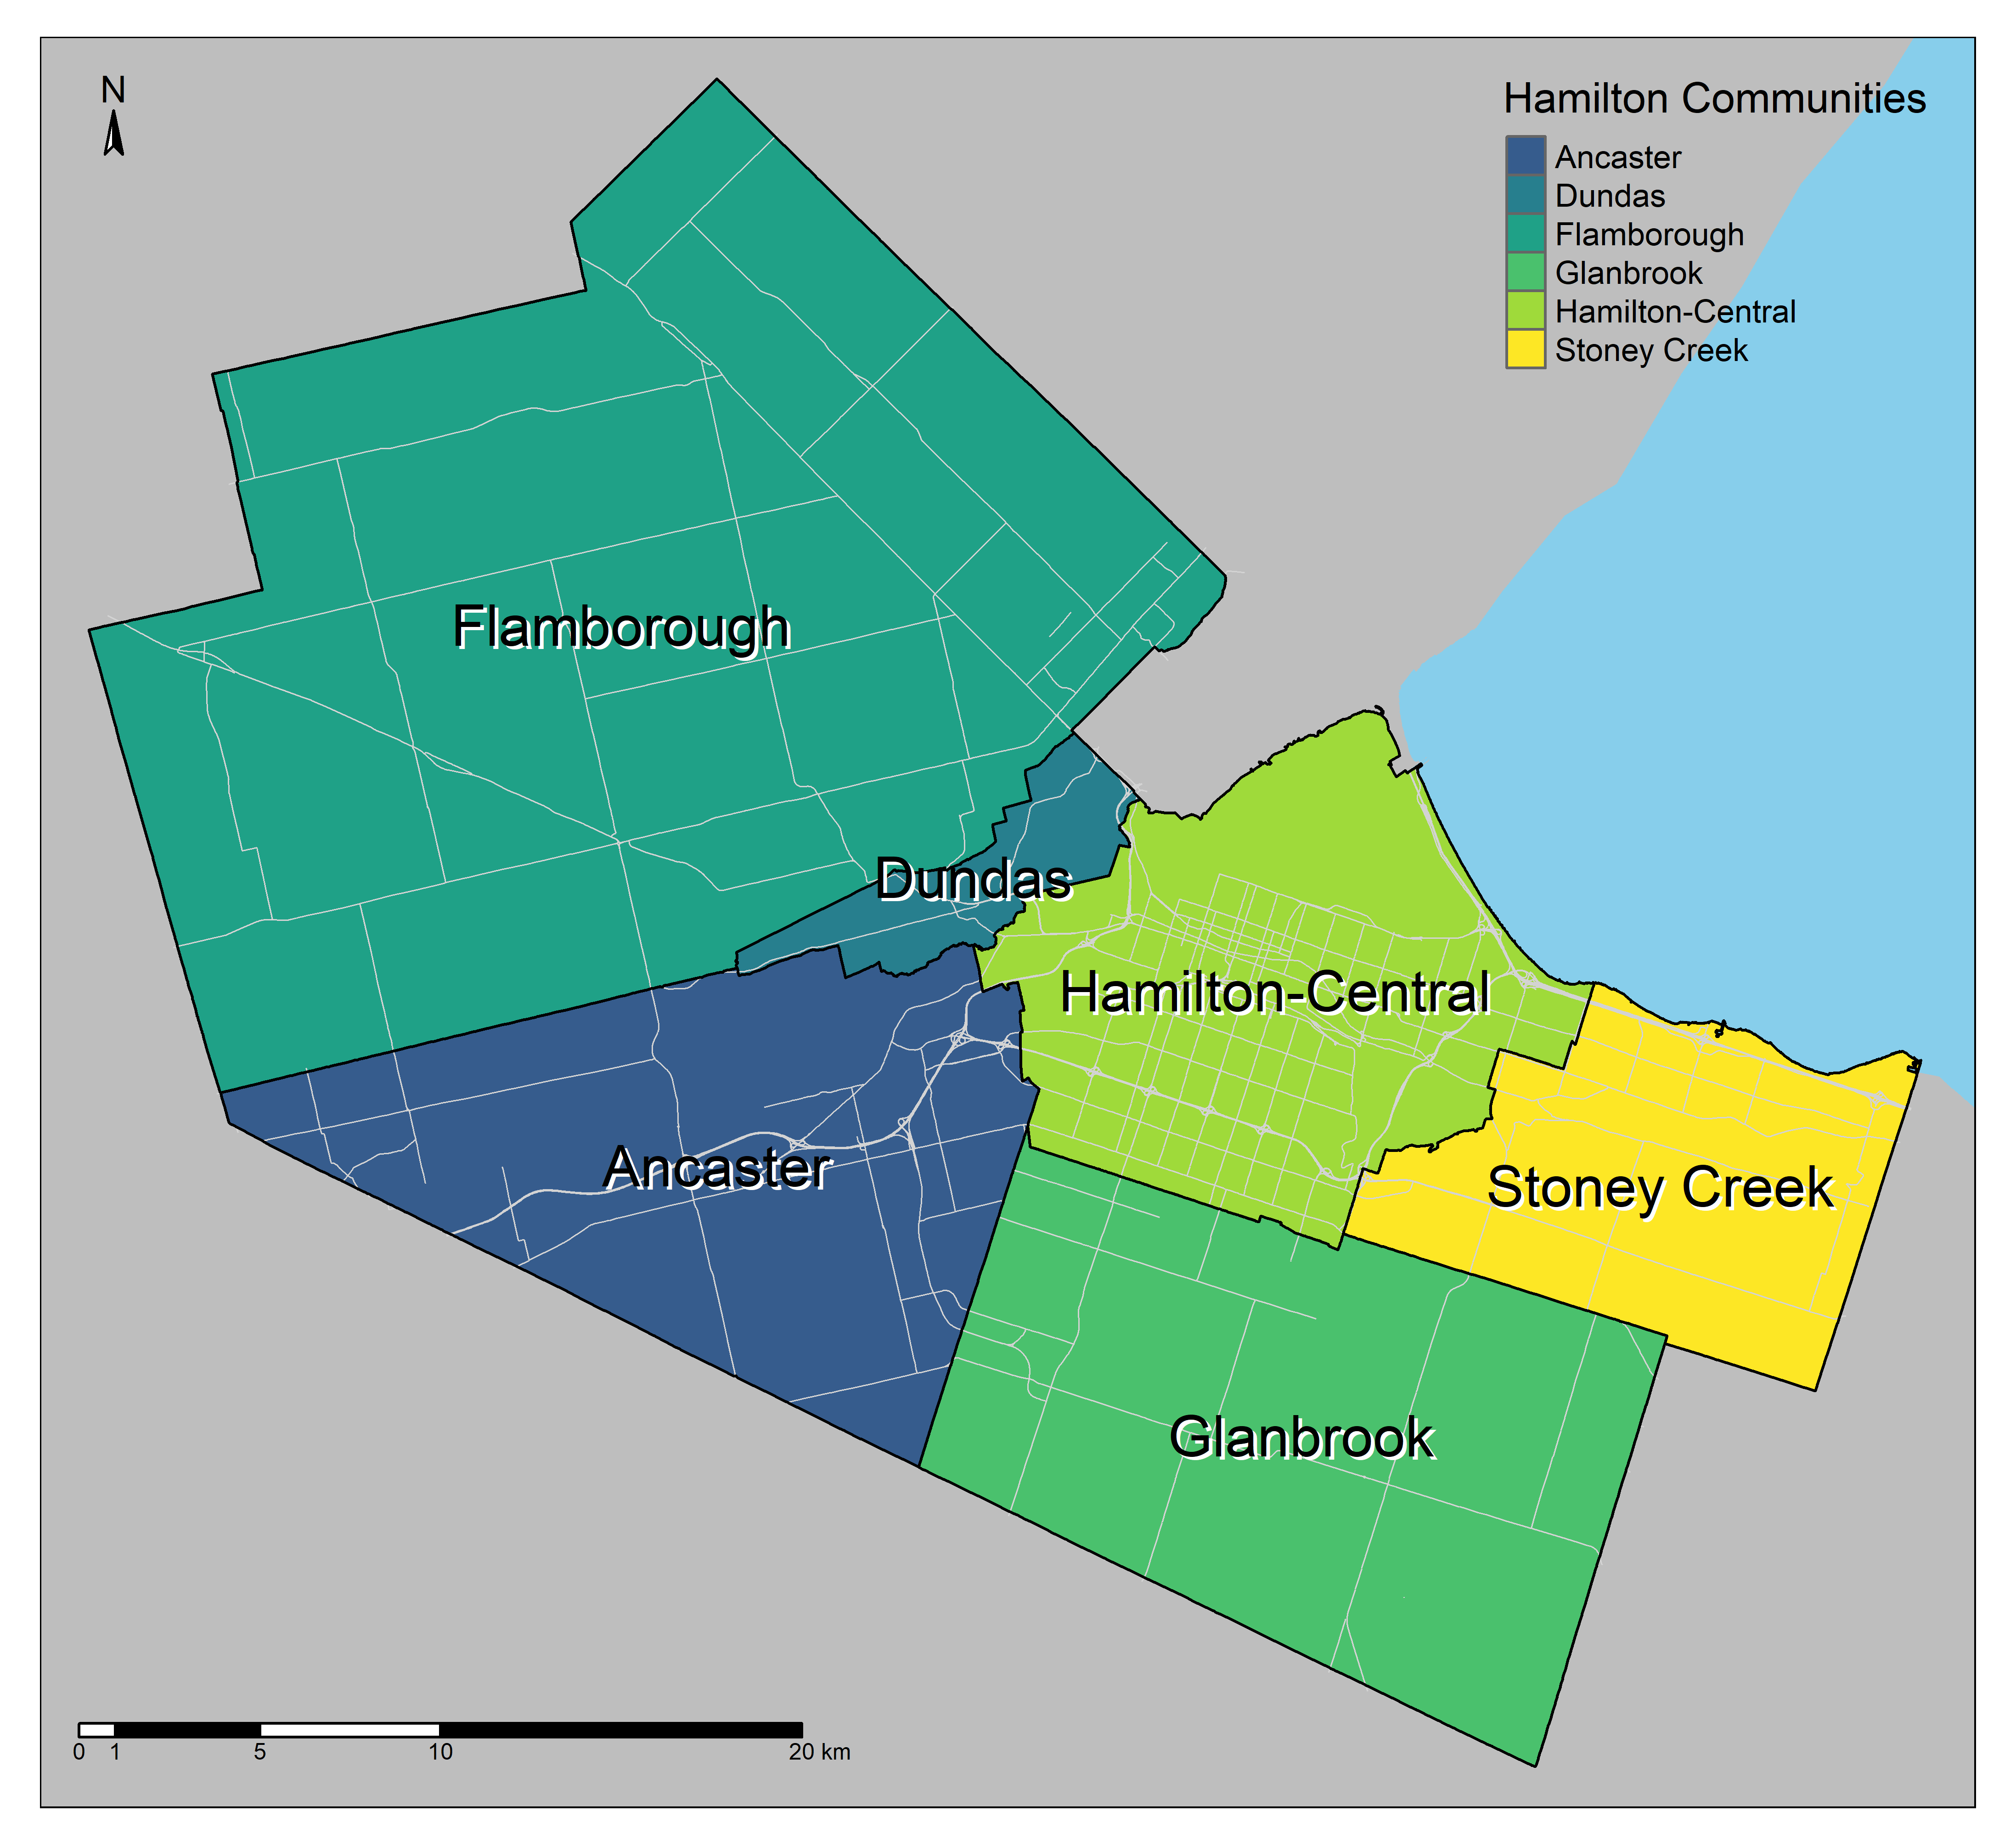
\includegraphics[width=6.25in,height=\textheight]{figures/Fig1-boundaries.png}

}

\caption{\label{fig-Fig1}The six former muncipal boundaries in the city
of Hamilton. Basemap shapefiles are retrieved from the Open Data
Hamilton Portal \citep{opendatahamiltonCityBoundary2023} and the USGS
\citep{greatlakesUSGS2010}. Highways and arterial roads are shown in
light grey.}

\end{figure}

\hypertarget{destination-database}{%
\subsection{Destination database}\label{destination-database}}

To complete the accessibility analysis, a geospatial database of care
destinations for Hamilton (e.g., full addresses of longitude and
latitude) was compiled. The geospatial data was sourced from
governmental open data portals
\citep{governmentofontarioOntarioDataCatalogue2023, cityofhamiltonOpenData2023},
Data Axle, a consumer database compiled of businesses and companies
within Canada \citep{axledataConsumerData2023} or manually through
Google Maps. Each destination was categorized based on the specific type
of care being accessed. Categories include child-, elder-, errand-,
grocery-, and health- centric destinations. These final categories, and
their sources of data, are described as follows and their spatial
distribution is visualized in Figure~\ref{fig-Fig2}.

\hypertarget{child-centric}{%
\subsubsection{Child-Centric:}\label{child-centric}}

This category includes the geospatial location of all child-oriented
destinations such as \textbf{schools}, \textbf{daycares},
\textbf{community centres}, \textbf{recreation centres}, and
\textbf{parks}: 1190 destinations are identified in the City.

\begin{itemize}
\tightlist
\item
  \textbf{Schools} are sourced from the Educational Institution data
  from Open Data Hamilton
  \citep{opendatahamiltonEducationalInstitutions2022}. The data was then
  filtered, and all locations that typically do not serve children were
  removed including: Post-Secondary, Adult-Learning Centres, Group
  Homes, and Foster Care Centres. Through examination some ``Section
  23'' institutions defined as \emph{``centres for children who cannot
  attend school to meet the needs of care or treatment, and
  rehabilitation''}
  \citep{governmentofontarioministryofeducationFundingEducationCommunity2023},
  were kept due to their innate connection to care.
\item
  \textbf{Daycares} were identified from the Registered Child Care
  Facilities in the Ontario Open Data Portal
  \citep{governmentofontarioOntarioDataCatalogue2023} and filtered to
  Hamilton. Additionally, EarlyON childcare locations, defined as
  \emph{``\ldots locations for child rearing and development where
  parents accompany their children''}
  \citep{cityofhamiltonChildCareRegistry2023}, were added manually from
  the Hamilton Child Care Registry
  \citep{cityofhamiltonChildCareRegistry2023}.
\item
  \textbf{Community centres}, \textbf{recreation centres}, and
  \textbf{Parks} were identified from the Recreation and Community
  Centres and Parks data from Open Data Hamilton
  \citep{opendatahamiltonParksDatabase2022, opendatahamiltonRecreationCommunityCentres2022},
  respectively.
\end{itemize}

\hypertarget{elder-centric-destinations}{%
\subsubsection{Elder-Centric
Destinations:}\label{elder-centric-destinations}}

This category includes the geospatial locations of \textbf{senior
centres}, \textbf{long-term care homes}, and \textbf{retirement homes}:
75 destinations are identified in the City. \textbf{Senior centres} are
also retrieved from the Recreation and Community Centre database
\citep{opendatahamiltonRecreationCommunityCentres2022}, specifically
locations that contain the name ``Senior Centre''. \textbf{Long-term
care homes} and \textbf{retirement homes} are sourced from the Ontario
Ministry of Health GEOHub for Health Service Locations
\citep{ontarioministryofhealthgeohubMinistryHealthService2023}.

\hypertarget{grocery-centric}{%
\subsubsection{Grocery-Centric:}\label{grocery-centric}}

This category includes the geospatial location of all \textbf{grocery
stores}, a place a household could buy groceries ranging from
convenience stores to large retail stores: 381 destinations are
identified. Data is gathered from Data Axle and filtered by Company
Name, Suite Number, Address, City, Province, Phone Number and Postal
Code \citep{axledataConsumerData2023}. From there the type was
identified e.g., grocers specialty foods, grocers retail, grocer health
food, grocer wholesale, grocer curbside, grocer delicatessen wholesale,
grocer convenience. Next, data was cross referenced to ensure all
included locations were operational and legitimate grocery stores.

\hypertarget{health-centric}{%
\subsubsection{Health-Centric:}\label{health-centric}}

This category includes the geospatial location of health destination
including \textbf{hospitals}, \textbf{pharmacies}, \textbf{clinics}, and
\textbf{dentist offices}: 421 destinations are identified in the City.
\textbf{Hospitals} and \textbf{pharmacies} were derived from the Ontario
Ministry of Health GEOHub for Health Service Locations
\citep{ontarioministryofhealthgeohubMinistryHealthService2023}.
\textbf{Clinics} were manually entered with data being gathered from
Hamilton Niagara Haldimand Brant Health Line -- Health Service Locations
\citep{hamiltonniagarahaldimandbranthealthlineWalkInMedicalClinics2023}.
Clinic data was then double checked to ensure locations were in
operation. Dentistry locations were also manually entered through Google
Map search filtering as well as reassessed for operational use.

\hypertarget{errand-centric}{%
\subsubsection{Errand Centric:}\label{errand-centric}}

This category includes other types of destinations that are
errand-centric such as \textbf{libraries}, \textbf{post offices}, and
\textbf{banks}: 158 destinations are identified in the City. In travel
surveys, these destinations are often lumped in within `grocery
shopping' \citep{taylorWhatExplainsGender2015}. In this research, we
distinguish these destinations from child-, elder-, grocery- and
health-centric destinations. \textbf{Libraries} are derived from
Hamilton Open Data Portal \citep{opendatahamiltonLibraries2022}.
\textbf{Post Offices} are collected from two sources; Axle Database and
then supplemented from the Canada Post Postal Office Tracker Website
\citep{axledataConsumerData2023, canadapostPostOfficeLocator2023}. The
supplemented locations from Canada Post Postal Office Tracker Website
were manually entered into the database to ensure data was accurately
being represented from its source. \textbf{Banks} are also derived from
Axle Data and then cross referenced to ensure data quality with the ABM
Bank Locator websites for the following national banking firms: Bank of
Montreal, CIBC, HSBC, National Bank of Canada, Royal Bank of Canada,
Scotiabank and TD Financial
\citep{bankofmontrealBankMontrealBranch2023, thehongkongandshanghaibankingcorporationlimitedhsbcHSBCBranchABM2023, nationalbankNationalBankBranches2023, royalbankofcanadaRBCBranchABM2023, scotiabankScotiabankABMBranch2023, thetorontodominionbankTDBankBranch2023}.

\begin{figure}

{\centering 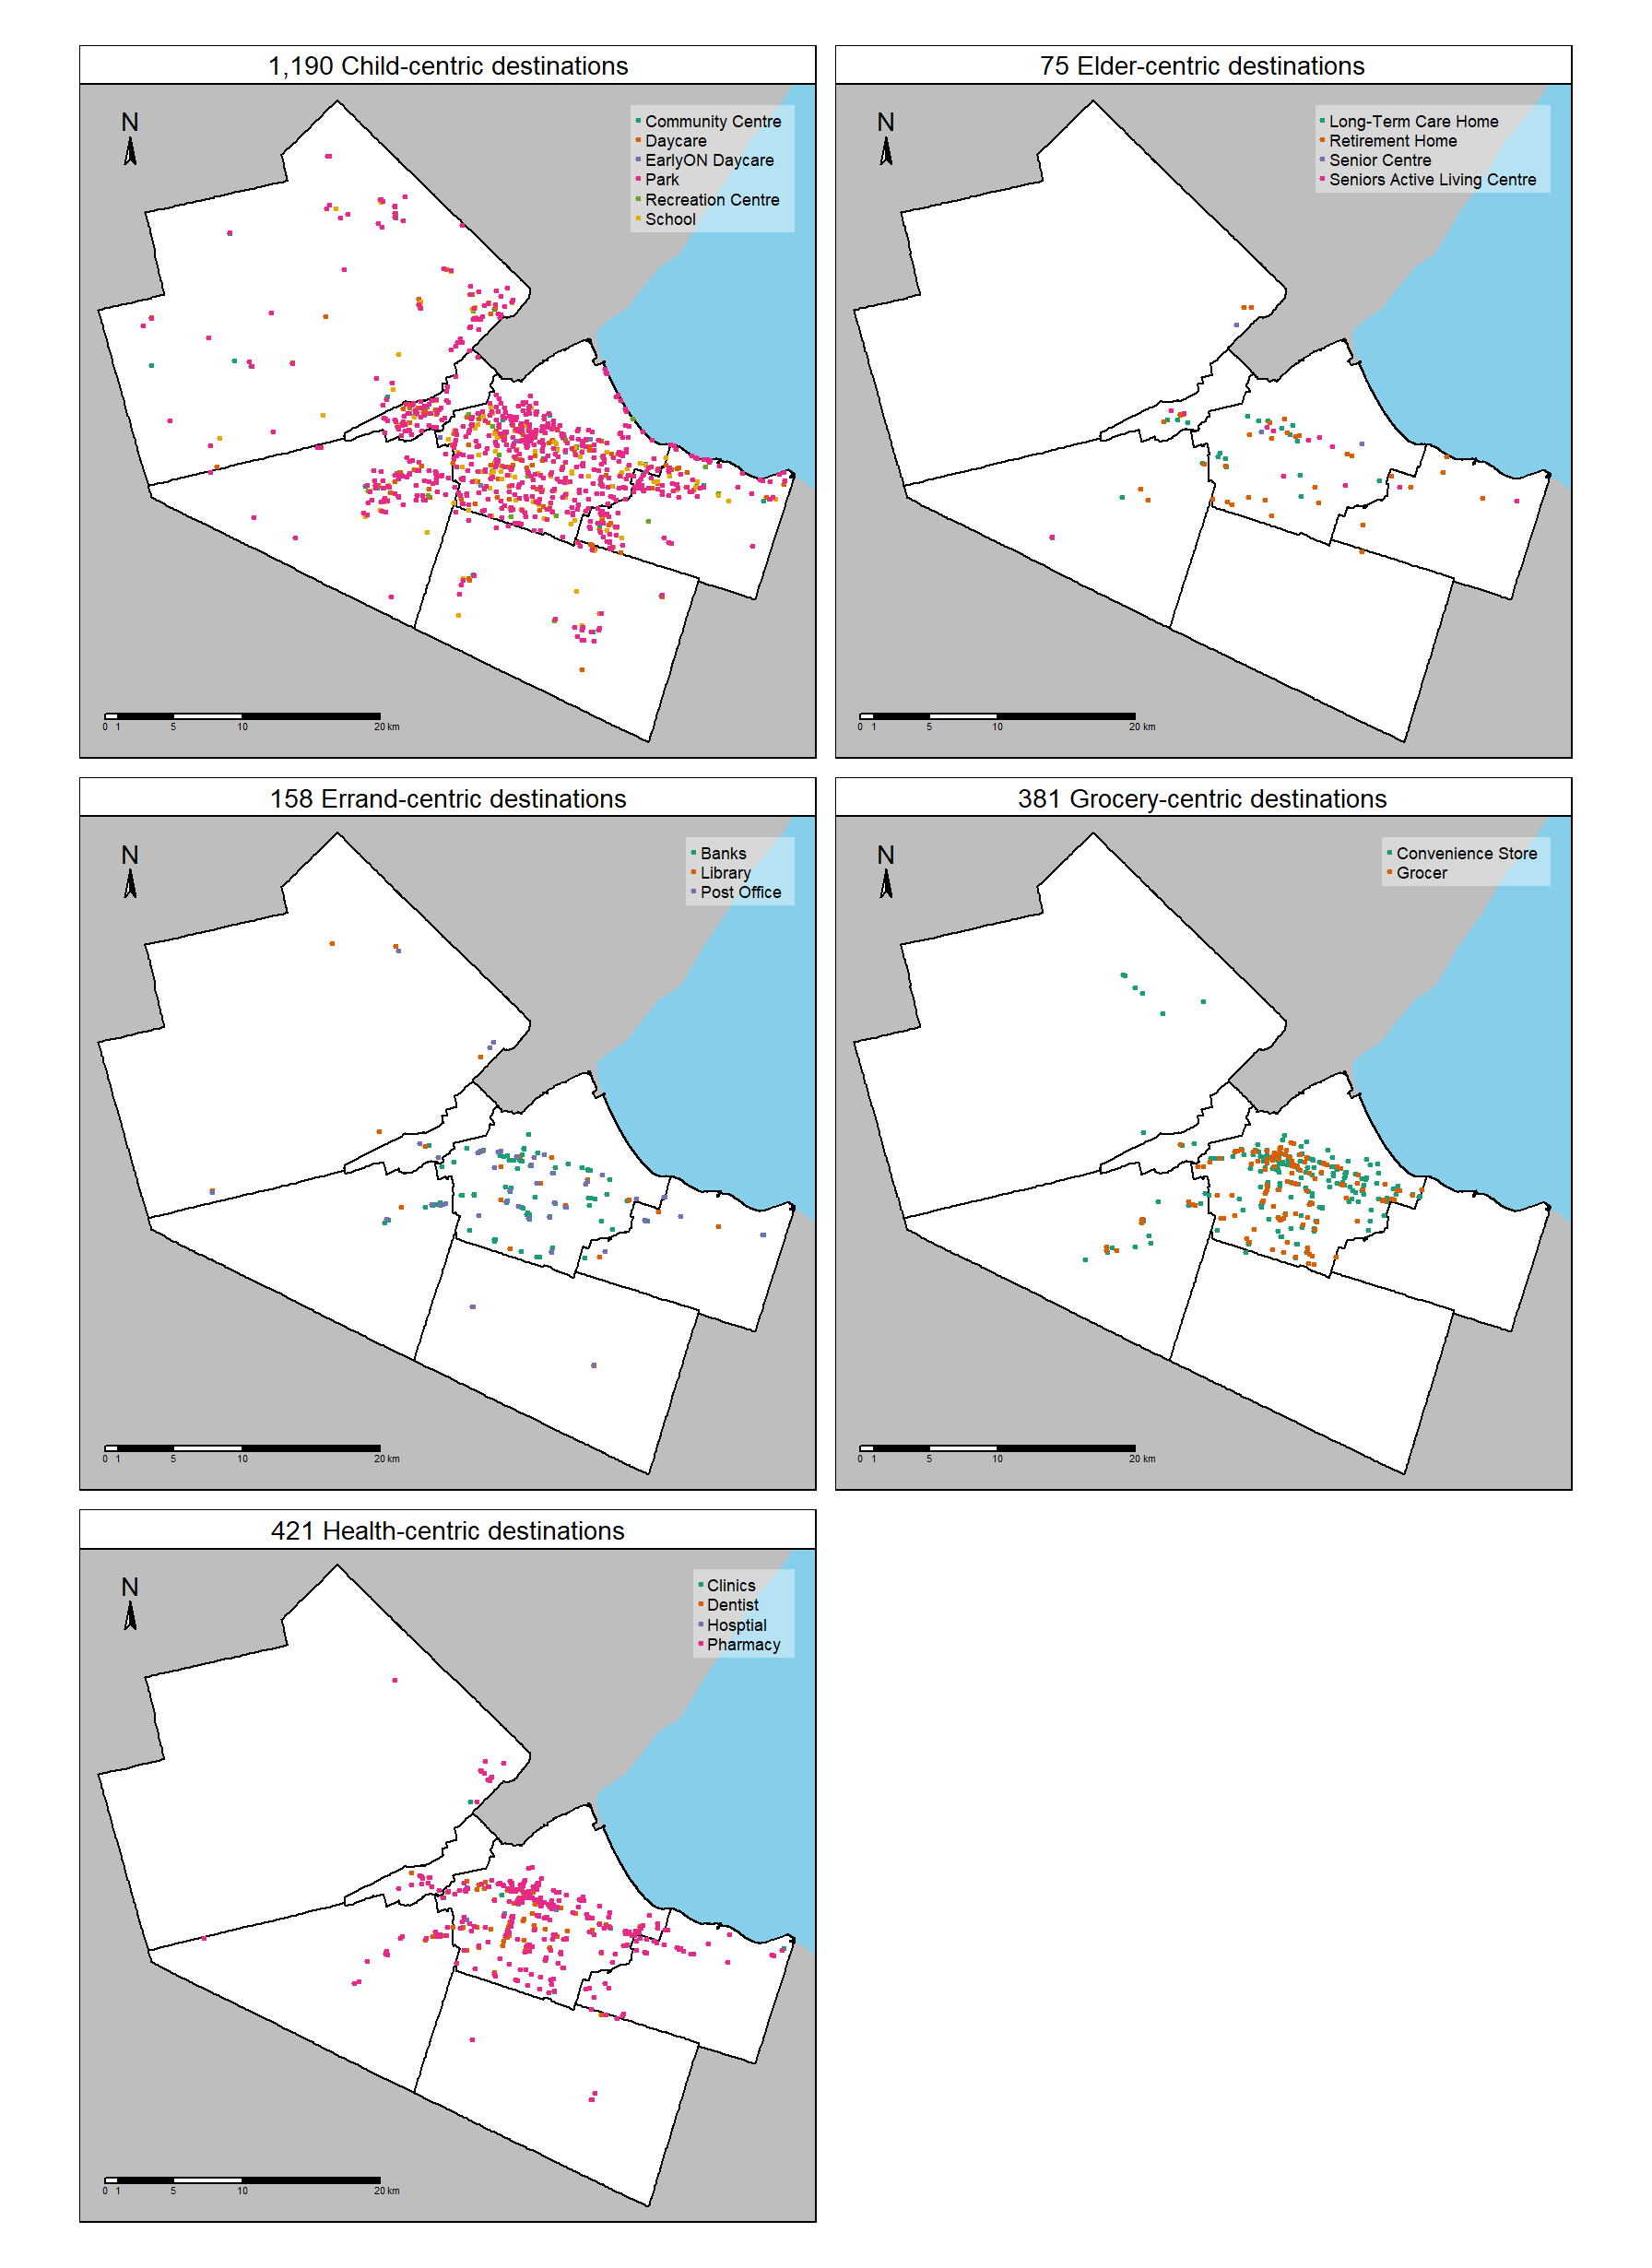
\includegraphics[width=6.25in,height=\textheight]{figures/Fig2-plot_care_categories.png}

}

\caption{\label{fig-Fig2}The geo-located points of care destinations in
the City of Hamilton separated by the author-generated categories of:
child-, elder-, errand-, grocery- and health- centric care categories.
Locations of these destinations were retrieved through multiple sources
as described in the text. Basemap shapefiles are sourced from the Open
Data Hamilton Portal \citep{opendatahamiltonCityBoundary2023} and the
USGS \citep{greatlakesUSGS2010}.}

\end{figure}

Once the care destinations were compiled, the data was validated to
ensure that duplicate locations were removed. Each location was manually
inspected using Google Maps to confirm if it was operational and
legitimate, if not, those locations were removed. The complete care
destination database was imported into RStudio for further processing
and visualised in Figure~\ref{fig-Fig2}, by category and sub-category.

For the purpose of this analysis and in absence of city-wide empirical
household preferences for care destinations, all destinations are
re-weighted to be equal. For example, if all count as 1 destination in
our analysis, the result will favour child-centric destinations as they
make up the majority of the database. As such, the five care categories
are re-weighted so they each represent one-fifth of the database:

\begin{itemize}
\tightlist
\item
  Child-centric (1190 destinations each at 0.3739496),
\item
  Elder-centric (75 destinations each at 5.9333333),
\item
  Errand-centric (158 destinations each at 2.8164557),
\item
  Grocery-centric (381 destinations each at 1.167979) and,
\item
  Health- centric (421 destinations each at 1.0570071) .
\end{itemize}

\hypertarget{census-data-and-multimodal-travel-time-estimations}{%
\subsection{Census data and multimodal travel time
estimations}\label{census-data-and-multimodal-travel-time-estimations}}

To supplement the care destination database and complete the
accessibility calculation, population data for the City of Hamilton was
sourced from the most recent 2021 Canadian census
\citep{governmentofcanadaCensusPopulation2023}. The number of residents
and the percent of after-tax low-income-cut-off (LICO-AT) residents was
sourced at the highest level of spatial resolution, the dissemination
area (DA). LICO-AT is a composite indicator included in the census that
reflects the proportion of households spending 20\% more than the area
average on food, shelter and clothing
\citep{governmentofcanadaLowIncomeCutoffs2023}. The \{cancensus\}
open-sourced R package was used to access the 2021 Canadian Census data
in a programmatic way \citep{vonbergmannCancensusCensusMapper2021}.
Figure~\ref{fig-Fig3} displays the spatial distribution of the total
population and the prevalence of LICO-AT as a percentage of the total
population. Of note is the density of population and LICO-AT prevalence
within Hamilton-Central.

\begin{figure}

{\centering 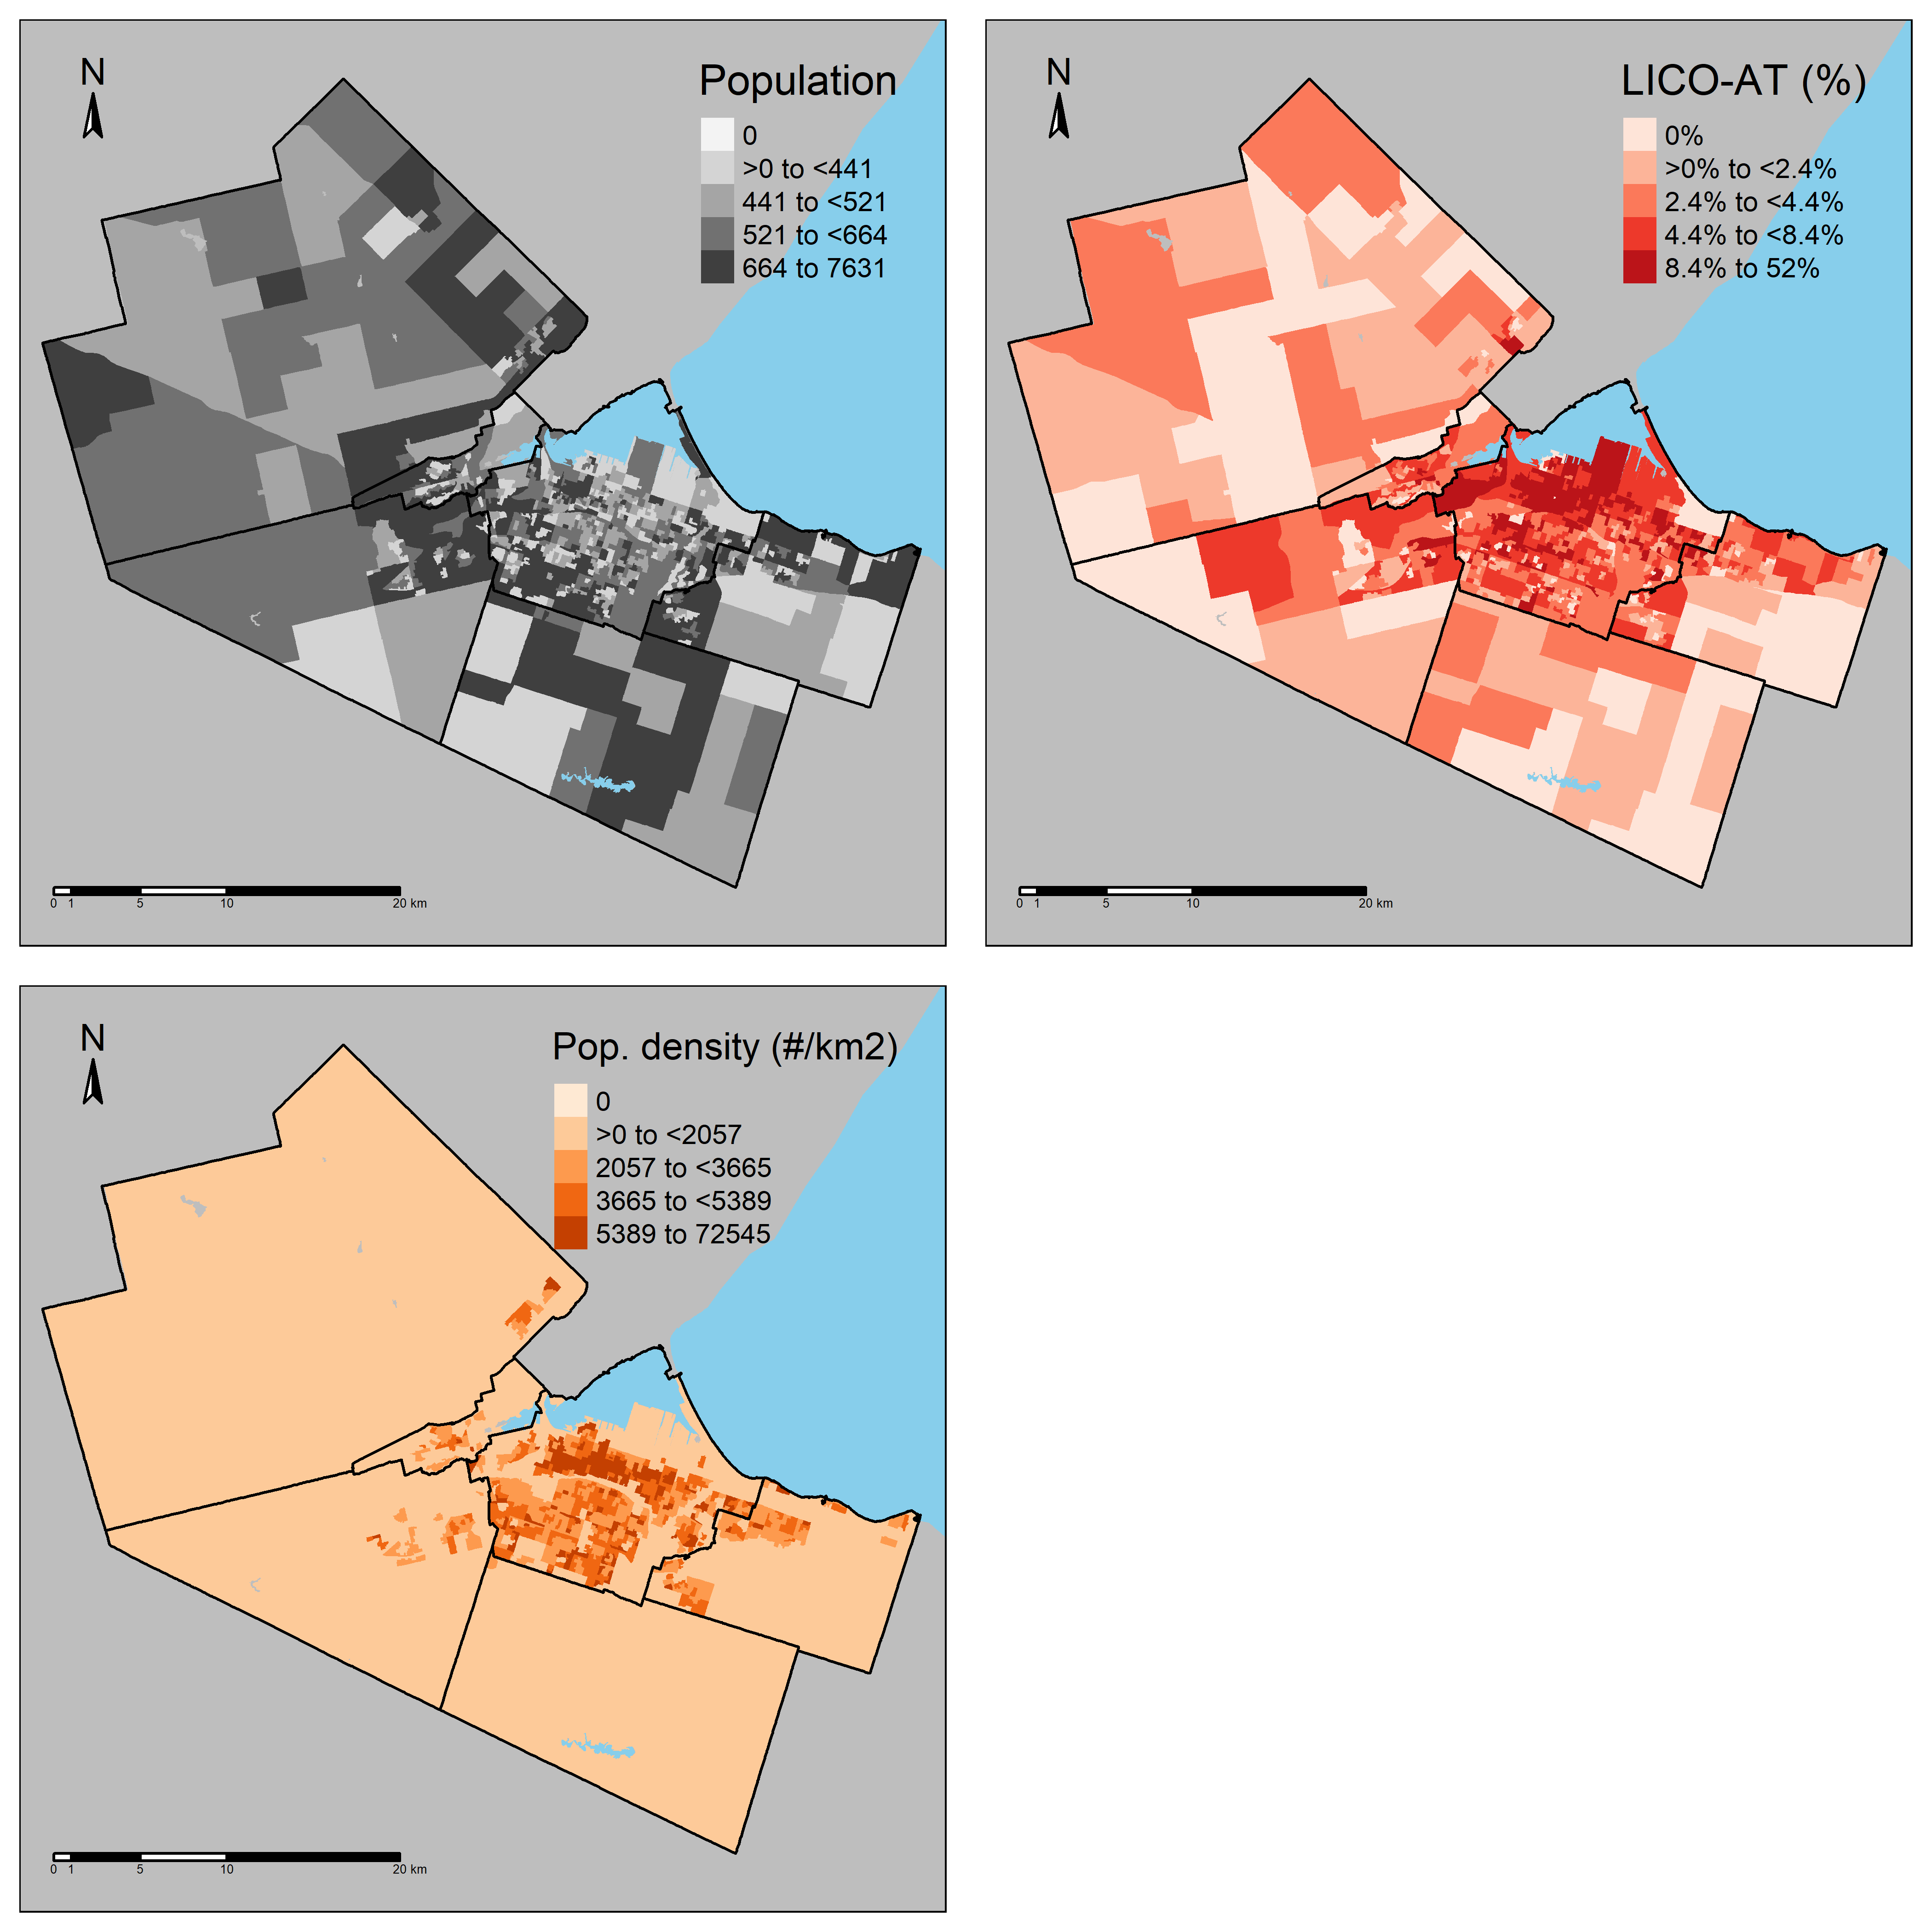
\includegraphics[width=6.25in,height=\textheight]{figures/Fig3-plot_pops.png}

}

\caption{\label{fig-Fig3}The total population in each dissemination area
(DA), visualized with the six former muncipal boundaries in the city of
Hamilton. The top plot represents the population density and the bottom
plot depicts the prevalence of low-income cutt-off after taxes (LICO-AT)
as a percentage of the total DA population. LICO-AT is a measure of
economic disadvantage. The legend categories represent quartiles.
Basemap shapefiles are retrieved from the 2021 Canadian census
\citep{governmentofcanadaCensusPopulation2023}, the Open Data Hamilton
Portal \citep{opendatahamiltonCityBoundary2023} and the USGS
\citep{greatlakesUSGS2010}.}

\end{figure}

To further investigate the spatial differences in access to care that
modes offer, we use the proportion of the total population that commute
by a specific mode (Figure~\ref{fig-Fig4}). These variables are also
retrieved as a long-form variable of the 2021 Canadian census using the
\{cancensus\} R Package
\citep{governmentofcanadaCensusPopulation2023, vonbergmannCancensusCensusMapper2021}.
Though mode-choice used in travel to work is not necessarily reflective
of the mode used to travel to care destinations, no other data is
available City-wide. That said, the population predominately commutes by
car, even within the more densely populated Hamilton-Central.

\begin{figure}

{\centering 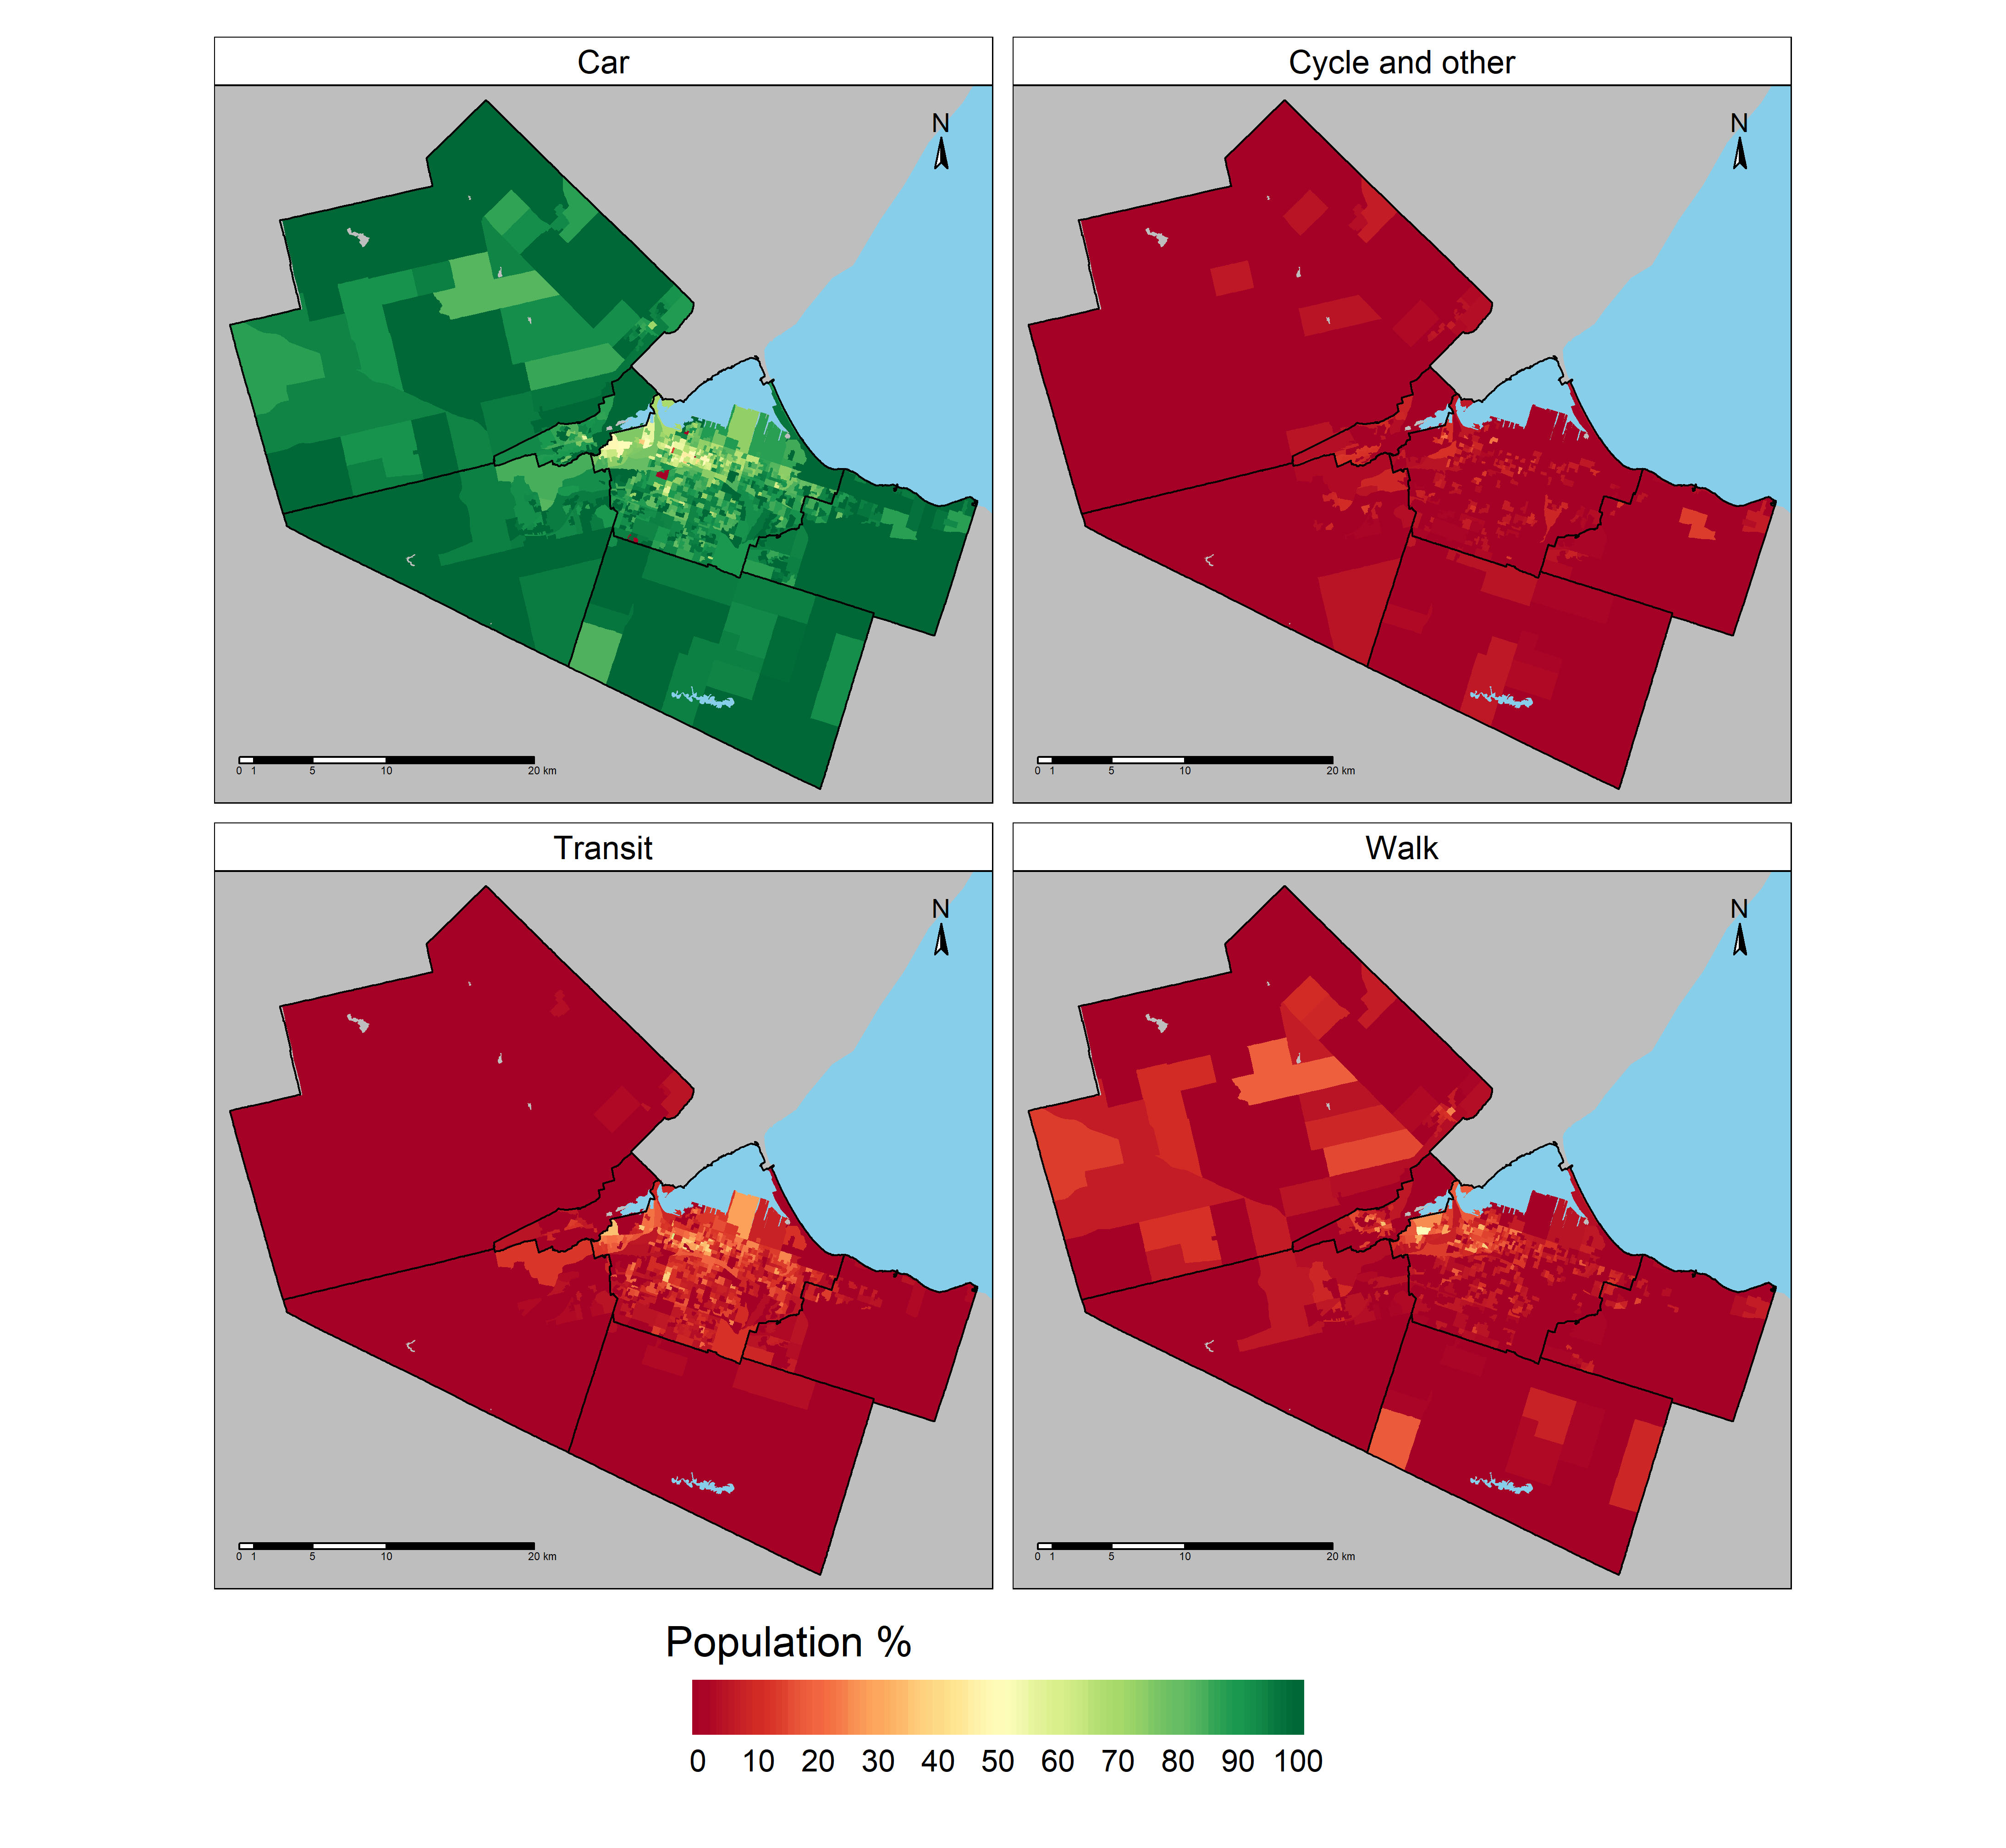
\includegraphics[width=6.25in,height=\textheight]{figures/Fig4-plot_modal_splits.png}

}

\caption{\label{fig-Fig4}The proportion of mode type used for commuting
(aged 15 and older employed in the labour force) in each dissemination
area (DA) as provided by the 2021 Canadian census. Basemap shapefiles
are retrieved from the 2021 Canadian census
\citep{governmentofcanadaCensusPopulation2023}, the Open Data Hamilton
Portal \citep{opendatahamiltonCityBoundary2023} and the USGS
\citep{greatlakesUSGS2010}.}

\end{figure}

Travel time is conducted using the `travel\_time\_matrix()' function
from \{r5r\}, an open-source R package for rapid realistic routing on
multimodal transport networks \citep{pereiraR5rRapidRealistic2021}. The
inputs were the geometric centroids of the DA, the centroids of all care
destinations, the Open Street Map (OSM) road network retrieved from
Geofabrik, \citep{geofrabrikOntarioCanadaOpen2023} and the static GTFS
(transit network in which only urban buses operate) for Hamilton
\citep{transitfeedsHamiltonStreetRailway2023}. Travel times for walking,
cycling, transit (with walking to stations), and car were calculated for
each origin to all care destinations.

For all modes, travel times under 60 minutes based on the shortest
travel-time path OSM road network were calculated. For transit and
cycling modes, additional parameters were included. In estimating
transit travel times, a typical Wednesday departure time at 8:00 was
selected, as it is representative of relative accessibility over the
course of the day \citep{boisjolyDailyFluctuationsTransit2016}. Further,
a departure travel window parameter of +/- 30 mins was used, so the
origin-destination travel times are calculated for each minute between
7:30 to 8:30. This consider is important as transit travel times are
highly sensitive to vehicle frequency and connecting transfers (see
discussion of the modifiable temporal unit problem e.g.,
\citep{pereiraFutureAccessibilityImpacts2019}). After evaluation, the
25th percentile travel time from the distribution of travel times in the
window was selected to represent each OD trip. This travel time
indicates that 25\% of trips from that origin to destination have a
travel time that is that length or shorter. This assumption provides an
optimistic assumption of transit travel times. For cycling travel times,
the default parameter for cycling routes of level 1 or 2 traffic level
of stress, dedicated or separated cycling lanes respectively, was
selected. The level of traffic stress is variable associated with links
of the OSM road network.

\hypertarget{accessibility-measures}{%
\subsection{Accessibility measures}\label{accessibility-measures}}

Both the \textbf{cumulative opportunity} and \textbf{spatial
availability} measure are used to estimate the potential access to care
that each mode provides to the DA. These measures represent the
aggregate zonal (DA) accessibility that populations that reside within
those DA may have access.

\textbf{Cumulative opportunity accessibility}: takes the following
general form for multi-mode calculation: \[
A_i^m=\sum_{j=1}^{J}O_j\cdot f^m(c_{ij}^m)
\] \noindent Where:

\begin{itemize}
\tightlist
\item
  \(i\) is a set of origin locations.
\item
  \(j\) is a set of destination locations.
\item
  \(m\) is a set of modes.
\item
  \(O_j\) is a number of opportunities at \(j\), in our case weighted.
\item
  \(c_{ij}^m\) is the travel cost between \(i\) and \(j\) for each
  \(m\).
\item
  \(f^m(\cdot)\) is an impedance function of \(c^m_{ij}\) for each
  \(m\); within the cumulative opportunity approach, it is a binary
  function that takes the value of 1 if \(c^m_{ij}\) is less than a
  selected value.
\item
  \(A^m_{i}\) is the unconstrained accessibility for \(m\) at each
  \(i\).
\end{itemize}

\textbf{Spatial availability} takes the following general form for
multi-mode calculation: \[
V^m_{i} = \sum_{j=1}^J O_j\ F^{tm}_{ij}
\] \noindent Where:

\begin{itemize}
\tightlist
\item
  \(i\), \(j\), and \(m\) is a set of origin locations, destination
  locations, and modes respectively.
\item
  \(O_j\) is a number of opportunities at \(j\), in our case weighted.
\item
  \(F^{tm}_{ij}\) is a balancing factor for each \(m\) at each \(i\). It
  depends on the size of the populations at different locations that
  demand opportunities \(O_j\), as well as the cost of movement in the
  system \(f(c_{ij})\).
\item
  \(V^m_{i}\) is the constrained accessibility (spatial availability)
  for \(m\) at each \(i\); the sum of \(V^m_{i}\) for all \(m\) at each
  \(i\) is equivalent to the total sum of opportunities in the region
  (i.e., \(\sum_j O_j = \sum_i V_i = \sum_{m} \sum_{i} V^m_{i}\)).
\end{itemize}

What makes spatial availability stand apart from other competitive
measures is the multimodal balancing factor \(F^{tm}_{ij}\) (discussed
in the pre-print by Soukhov et al.
\citep{soukhovMultimodalSpatialAvailability2023}). \(F^{tm}_{ij}\)
implements a proportional allocation mechanism that ensures the sum of
all spatial availability values at each \(i\) always matches the total
number of opportunities in the region. \(F^{tm}_{ij}\) consists of two
parts: the first is a population-based proportional allocation factor
\(F_i^{pm}\) that models the mass effect of the gravity model and the
second is an impedance-based proportional allocation factor
\(F_{ij}^{cm}\) that models the cost effect. Both factors consider
competition: \(F^{pm}_{i}\) estimates a proportion of how many people
are in each \(i\) and using each \(m\) relative to the region and
\(F^{cm}_{ij}\) estimates a proportion of the cost of travel from \(i\)
to \(j\) at each \(i\) using each \(m\) relative to the region. As both
\(F^{pm}_{i}\) and \$F\^{}\{mc\}\emph{\{i\} \$ are proportions,
\(\sum_{m} \sum_{i} F^{pm}_{i} = 1\) and \$ \sum}\{m\} \sum\emph{\{i\}
F\^{}\{cm\}}\{i\} = 1\$). Both factors are combined to equal the total
balancing factor \(F^{tm}_{ij}\) which is used to calculated \(V^m_i\)
as follows:

\[
F^{tm}_{ij} = \frac{F^{pm}_{i} \cdot F^{cm}_{ij}}{\sum_{m=1}^M \sum_{i=1}^N F^{pm}_{i} \cdot F^{cm}_{ij}}
\] \noindent Where:

\begin{itemize}
\tightlist
\item
  The factor for allocation by population for each \(m\) at each \(i\)
  is \(F^{pm}_{i} = \frac{P_{i}^m}{\sum_{m}\sum_{i} P_{i}^m}\). This
  factor makes opportunities available based on demand. The pop
\item
  The factor for allocation by cost of travel for each \(m\) at \(i\) is
  \(F_{ij}^{cm} = \frac{f^m(c_{ij}^m)}{\sum_{m} \sum_{i} f^m(c_{ij}^m)}\).
  This factor makes opportunities available preferentially to those who
  can reach them at a lower cost.
\end{itemize}

The use of both constrained and unconstrained accessibility measures is
strategic, as they illuminate different trends. As an unconstrained
measure, cumulative opportunity measure counts all the destinations that
can be reached from each DA within a travel cost, for each DA. From a
region-wide perspective, a destination that can be reached by multiple
DAs is counted multiple times, so the sum of all cumulative opportunity
values region-wide is not meaningful. However, cumulative opportunity
measure is relative straightforward to implement, and has been widely
used in accessibility research because of its simple computation (XX).
The value is understood relative to the score in the region, XX
opportunities can be accessed within 30 minutes from this neighbourhood
- this is XXth percentile in the estimated region, a regionally high
score. Comparisons of score within the region make sense, but
substantive interpretation of levels of access between modes is hard to
compare. We often seen, car provides more unconstrained access to
opportunities than transit.

On the other hand, spatial availability is constrained
\citep{soukhovIntroducingSpatialAvailability2023}, it incorporates the
concept of the \emph{finite}. The spatial availability value for each
mode at each DA is a count of how many destinations can be accessed by
that mode out of all the destinations in the region. The sum of spatial
availability values across the region is constrained to equal the total
number of opportunities. Proportions of each destination (supply) are
allocated to each mode at each DA based on the DA-to-region-relative
population (demand for opportunities) and travel impedance (travel cost
to opportunities). Unlike cumulative opportunity measure, multimodal
spatial availability measures can be used to extra additional meaning
between modes. It can be used to illustrate in what neighbourhoods do
car-drivers access \emph{more} than their equal share of opportunities
than transit-users and how much more, for instance.

The travel impedance threshold used in both measures is 15 minutes and
30 minutes; each measure is calculated eight times, once for each four
modes and assuming a travel time cut-off of 15 minutes or less and
another assuming a travel time cut-off of 30 minutes or less. The
selection of the travel time threshold was informed by the literature.
Only one study to date has calculated the average travel time to all
different categories of care destinations (16 minutes by car and 36 by
public transport) \citep{grantsmithManagingChallengesCombining2016}.
Other literature on travel to care trends to consider trips to one type
of care category (e.g., health, or school, or grocery stores). Here,
travel times vary by care category (e.g., 15 minutes to grocery shopping
\citep{hamrickTimeCostAccess2012} or 20.45 for cancer treatments
\citep{segelRuralurbanDifferencesAssociation2020}. In other care-related
accessibility analyses, time-cut offs include 10 mins (for daycares)
\citep{fransenCommuterbasedTwostepFloating2015} and 30 mins to 1 hr (for
hospitals) \citep{schuurmanDefiningRationalHospital2006}. Furthermore,
the use of a binary travel time threshold was selected, as opposed to
more complex impedance functions, to simplify computation. As mentioned,
region-specific empirical travel data regarding care-centric trip travel
times is lacking, and this work establishes a methodology to streamline
access to care interpretation and analysis for then that data is
available (?).

\hypertarget{results}{%
\section{RESULTS}\label{results}}

In absence of people's travel behaviour and preference for care
destinations - a bias in traditional travel surveys - we map access to
all destinations assuming an equal weighting of the five categories. The
results are described across: unconstrained access to care by mode
across the city, constrained access by mode, and identification of
intervention areas through equity considerations.

The cumulative opportunity accessibility plots for each mode are shown
in Figure~\ref{fig-Fig5}. It visualises an unconstrained count of
destinations, we can interpret it as: the more destinations that can be
reached by a mode, the more potential interactions and thus the
potentially better. Spatial trends between the 15 minute and 30 minute
threshold plots are similar (values are coloured by quantile). We can
also notice three significant findings between modes: first, the access
that car provides is significantly higher relative to other modes, it
sets the max. value of (1939 opportunities for 15 min and 2209
opportunities for 30 mins) across all modes. Next, access by cycling is
surprisingly also relatively high. And importantly, transit and walking
access is great and pretty good, respectively, within Hamilton-Centre
but this is not the same story in other communities.

\begin{figure}

{\centering 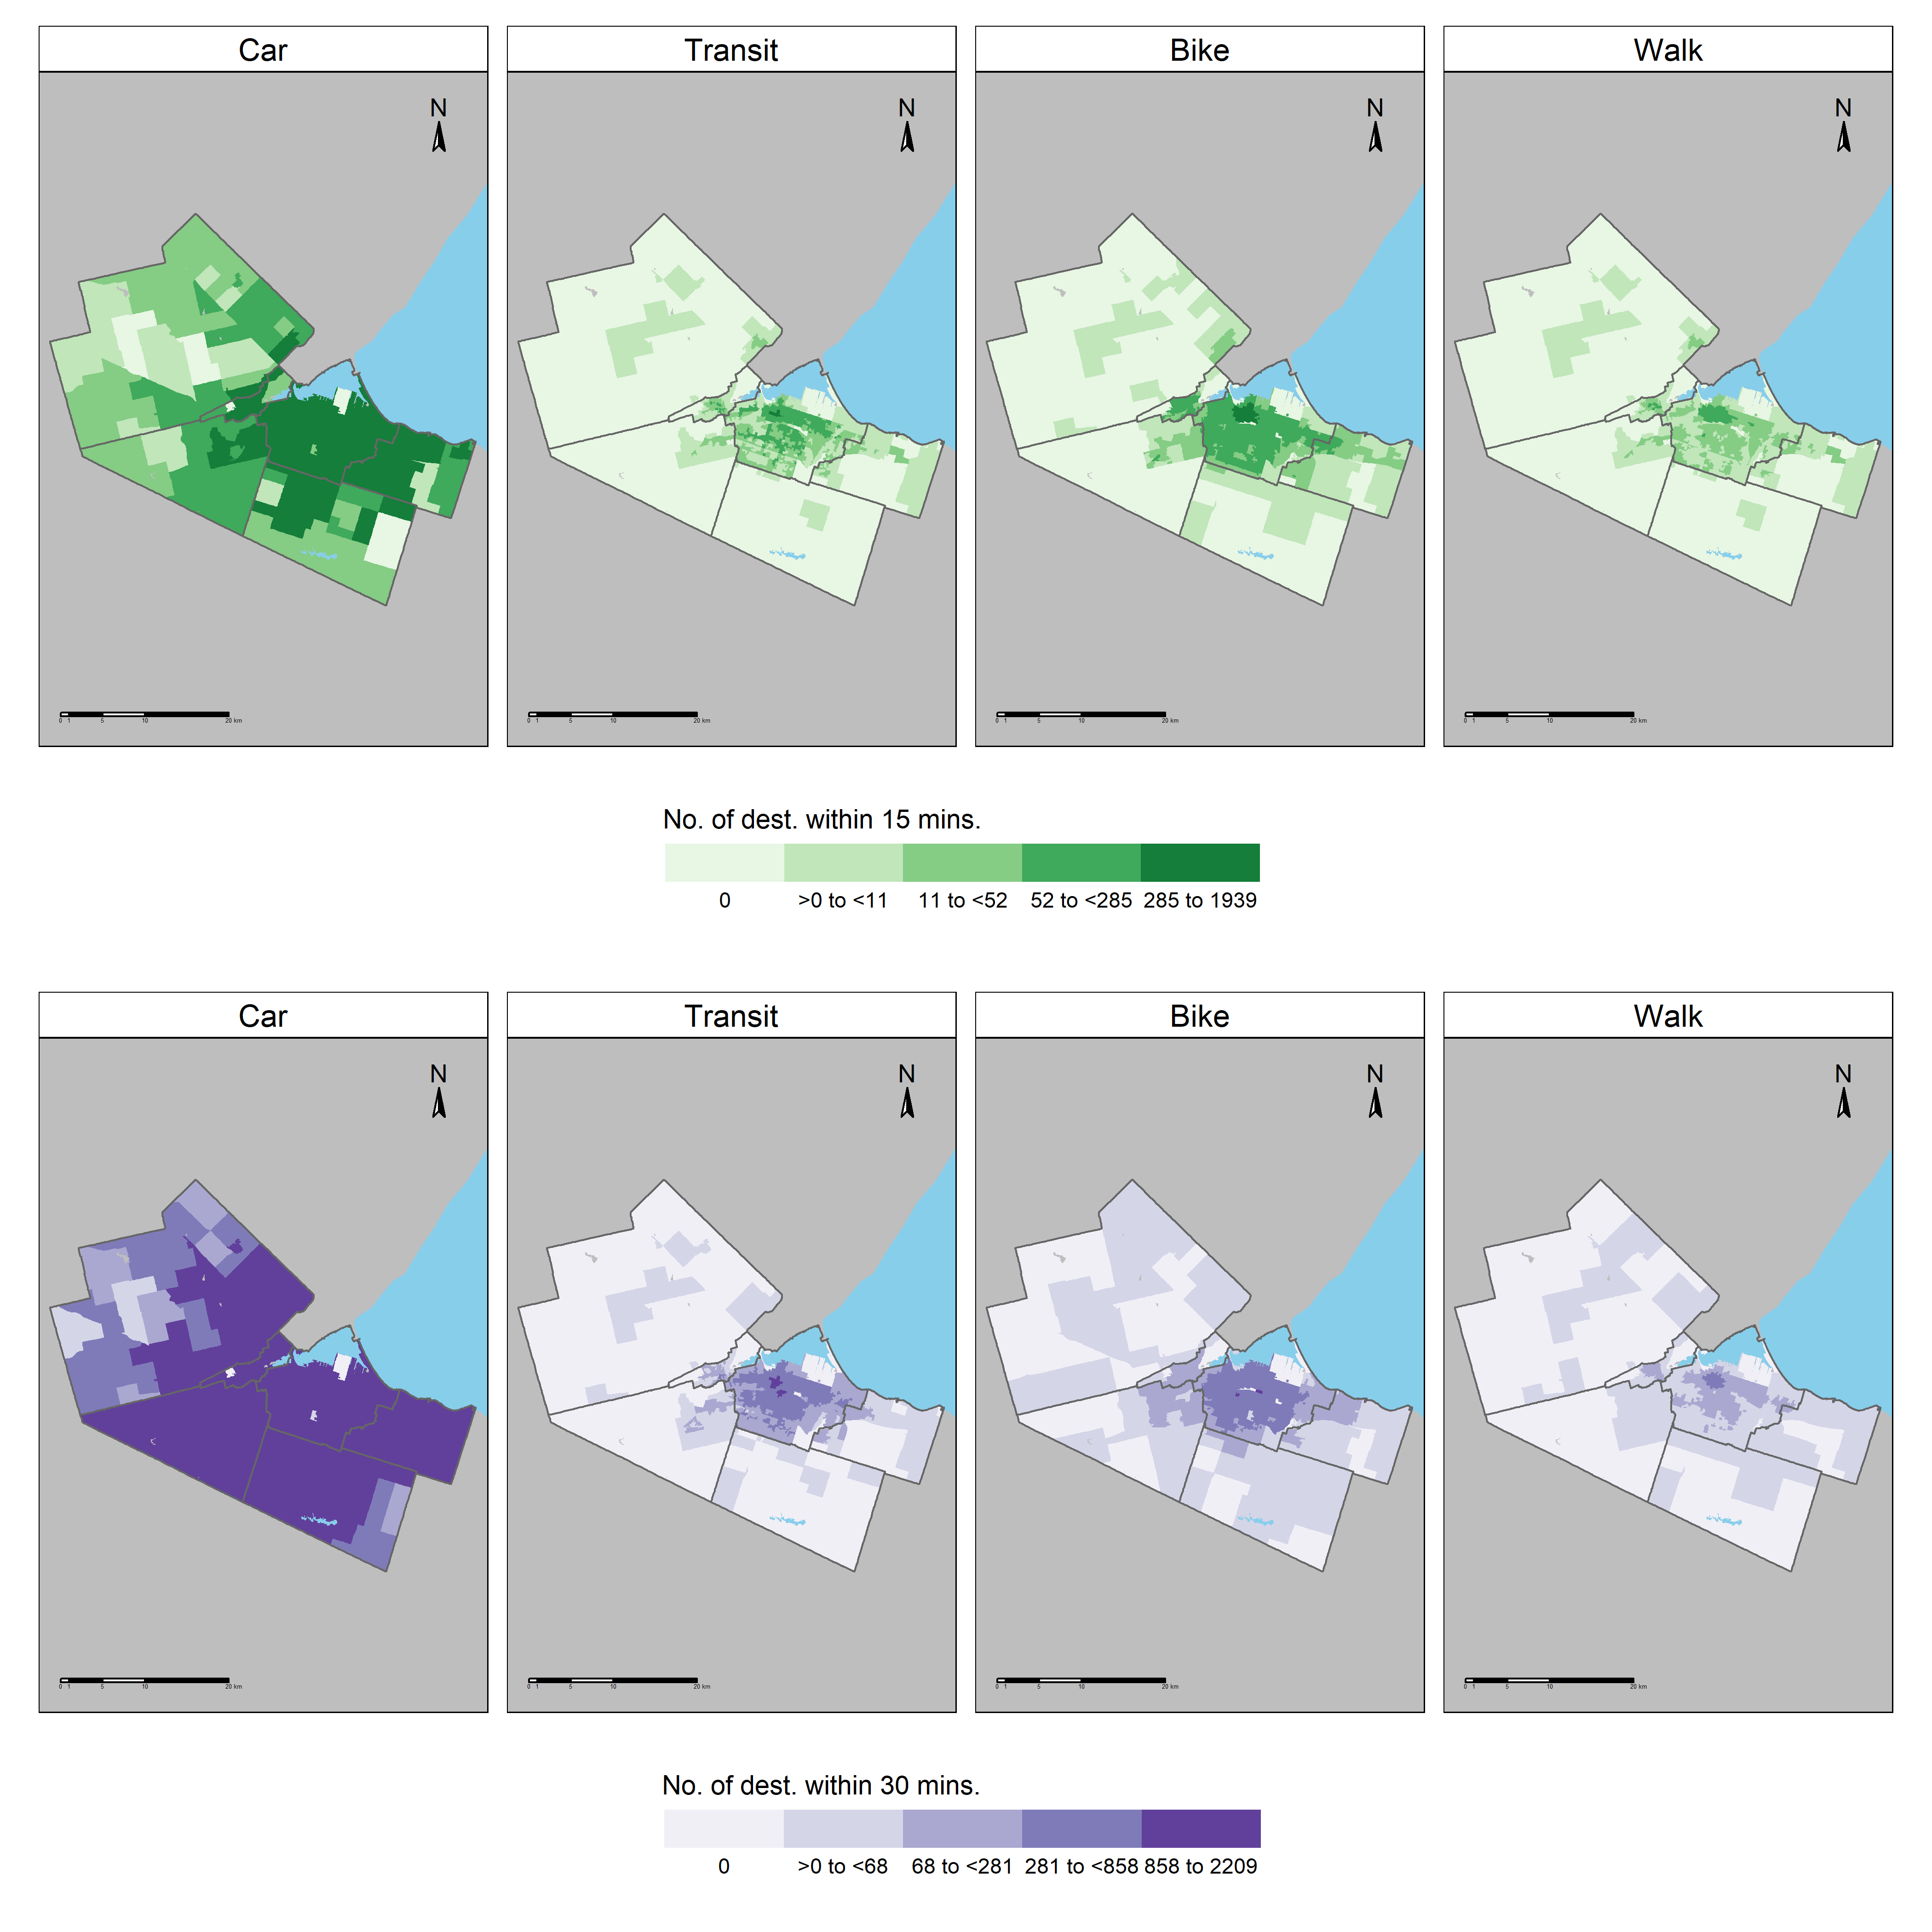
\includegraphics[width=6.25in,height=\textheight]{figures/Fig5-plot_cum_opp_measures.png}

}

\caption{\label{fig-Fig5}The cumulative opportunity measure. The number
of care destinations that can be reached, per DA, within 15 mins (top)
and 30 mins (bottom). Basemap shapefiles are retrieved from the 2021
Canadian census \citep{governmentofcanadaCensusPopulation2023}, the Open
Data Hamilton Portal \citep{opendatahamiltonCityBoundary2023} and the
USGS \citep{greatlakesUSGS2010}.}

\end{figure}

From Figure~\ref{fig-Fig5}, we can tell car is king, an expected outcome
given the tendency of North American cities to be designed around the
private car \citep{saeidizandRevisitingCarDependency2022}. However,
access by non-car modes is great (Q3 and Q4) within many DAs in
Hamilton-Centre and cycling has potential, especially in the more rural
communities (Q1). However, though many households use car as a commute
mode, not everyone does, wants to, or can. How does the access that car
provides \emph{out compete} access given by other modes? Lets consider
cycling. Though cycling provides access to many destinations, seeing the
2225 care destinations in the City as the total, how many of those are
potentially available to cyclists considering motorists greater
unconstrained access? We can't answer this question using unconstrained
accessibility, so lets turn to constrained accessibility, shown in
Figure~\ref{fig-Fig6}.

\begin{figure}

{\centering 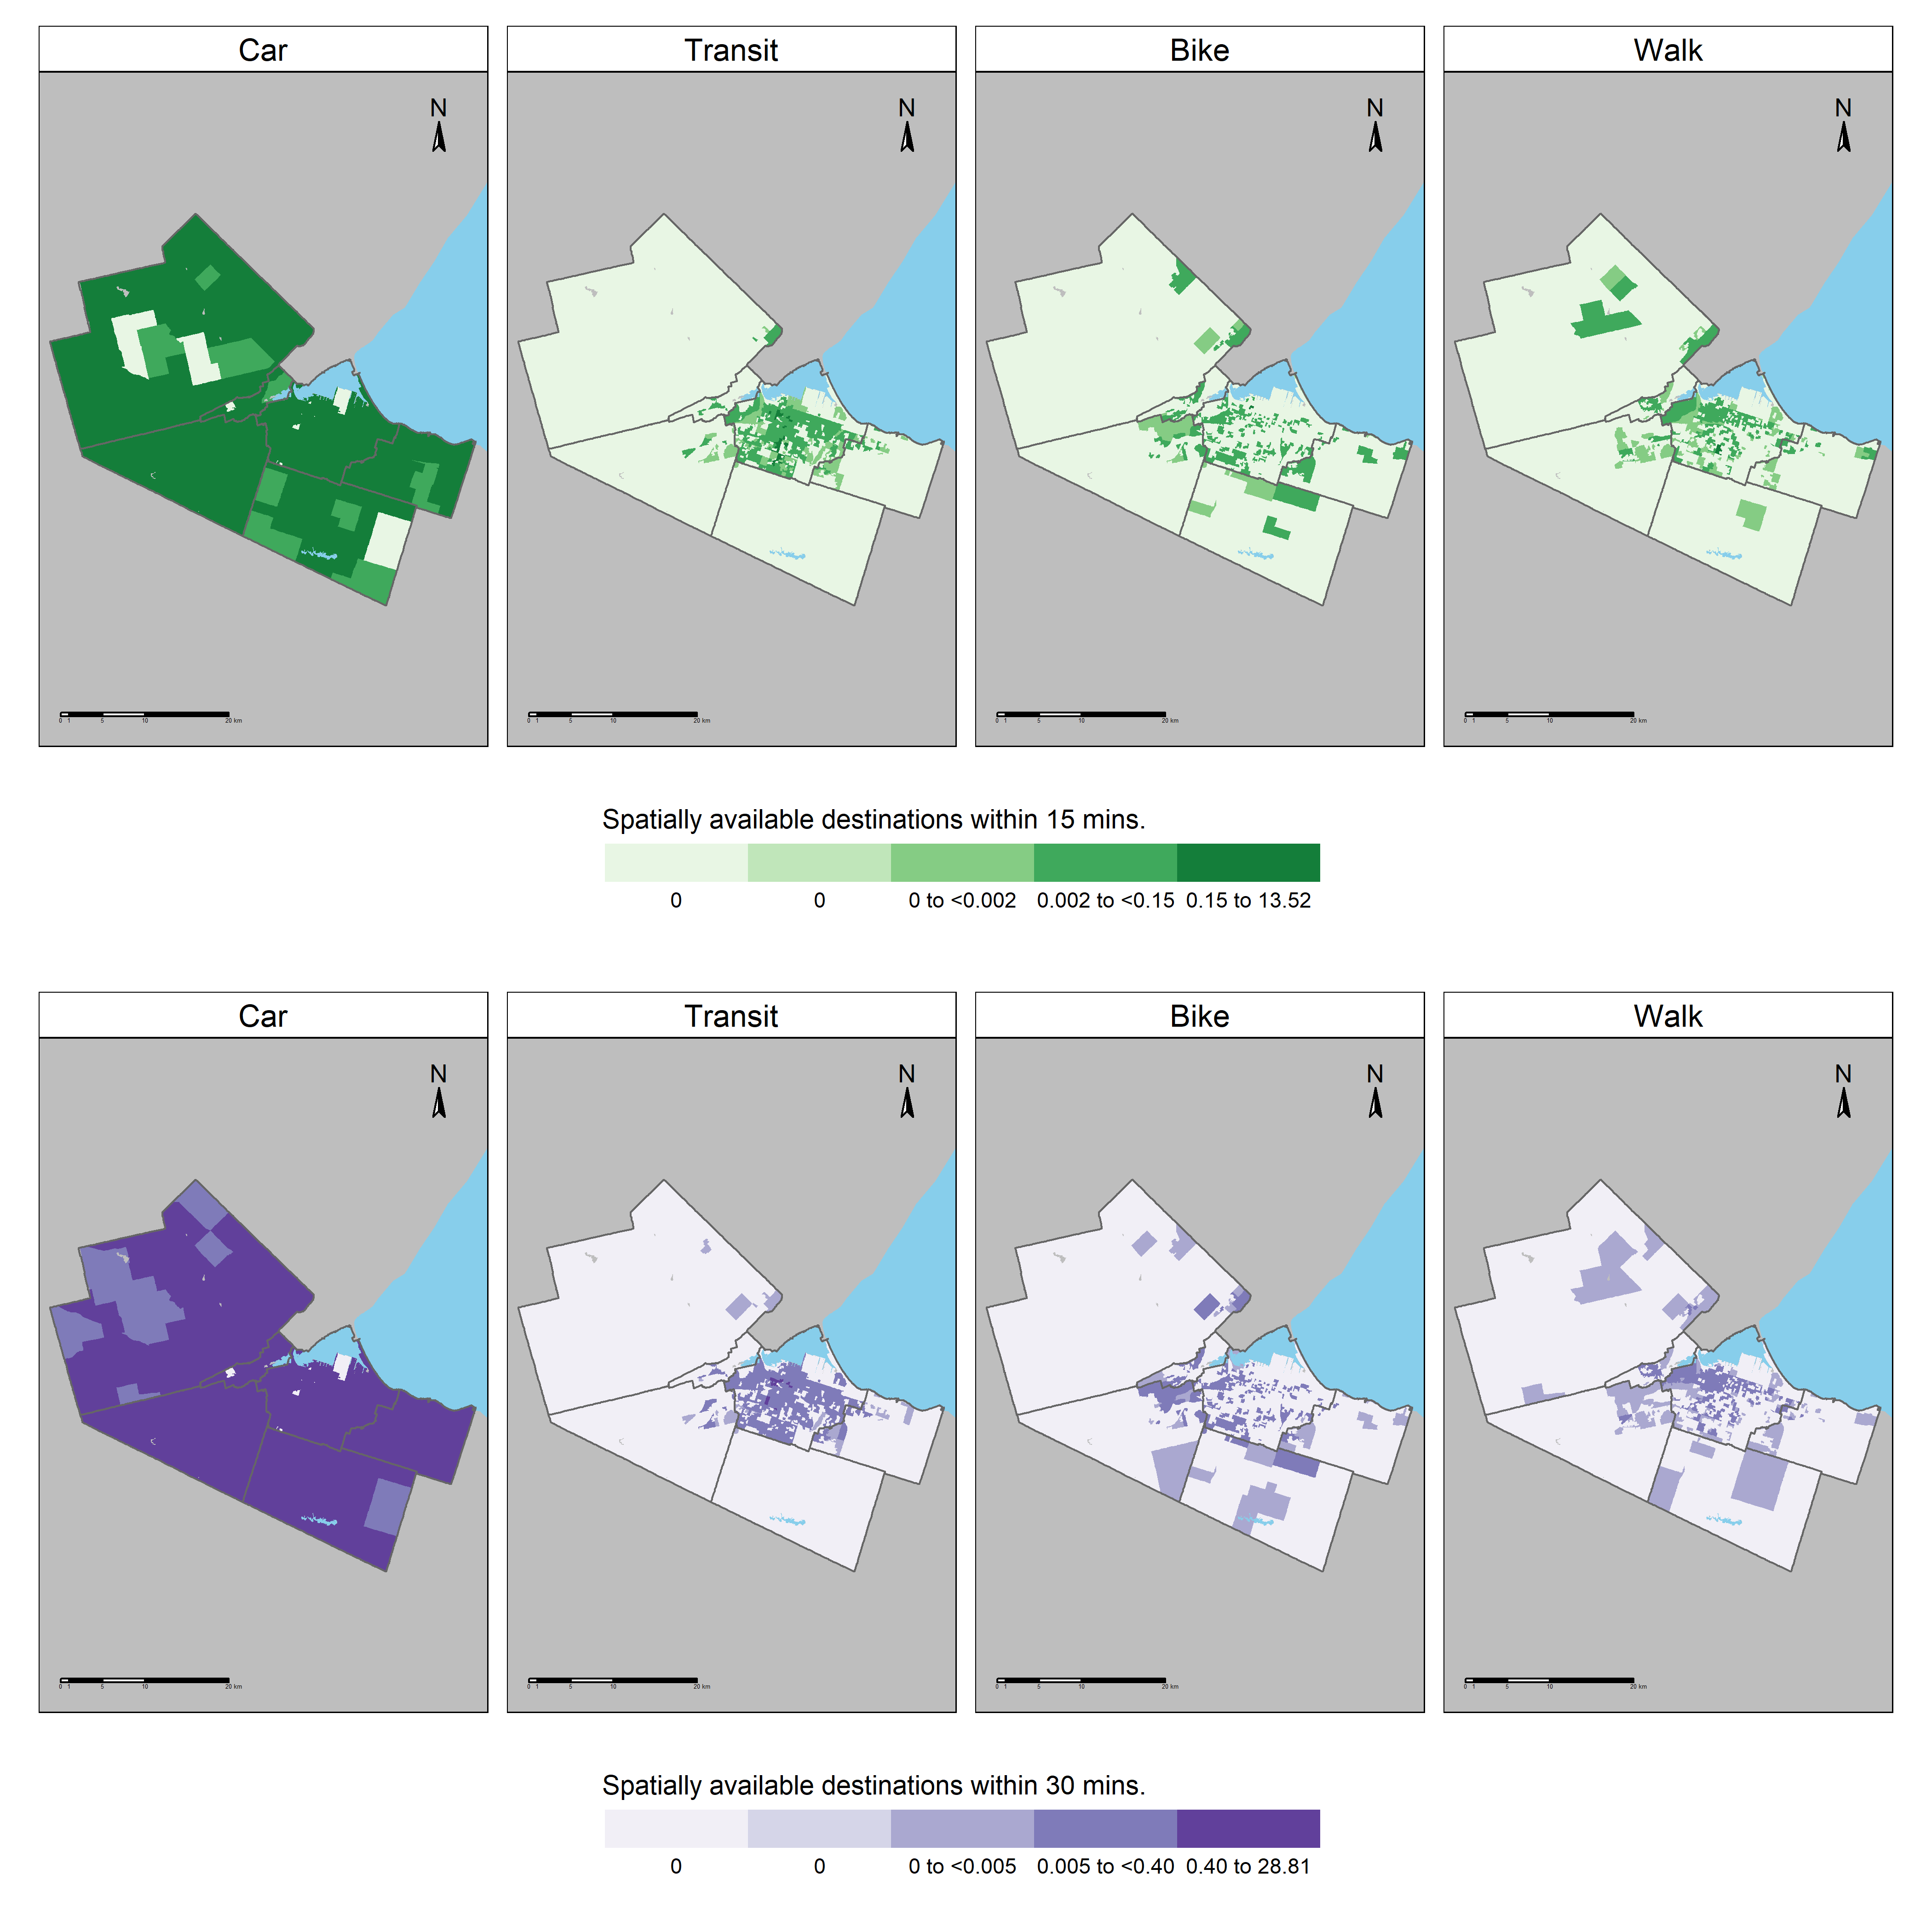
\includegraphics[width=6.25in,height=\textheight]{figures/Fig6-plot_Savail_measures.png}

}

\caption{\label{fig-Fig6}The spatial availability measure. The number of
care destinations that can be reached, per DA, within 15 mins (top) and
30 mins (bottom). Basemap shapefiles are retrieved from the 2021
Canadian census \citep{governmentofcanadaCensusPopulation2023}, the Open
Data Hamilton Portal \citep{opendatahamiltonCityBoundary2023} and the
USGS \citep{greatlakesUSGS2010}.}

\end{figure}

Assuming the population that commutes by a certain mode
(Figure~\ref{fig-Fig4}) also accesses care destinations by this mode,
the spatial availability per mode is displayed in Figure~\ref{fig-Fig6}.
We can observe that motorists capture the most \emph{availability} i.e.,
potential access to destinations out of all destinations. This is
in-part because many DAs, especially in rural communities, have 0\% or
exceptionally low non-car mode usage. From Figure~\ref{fig-Fig5} we can
see that non-car modes have potential, especially cycling, but
Figure~\ref{fig-Fig6} affirms that even though non-car modes may provide
good access within Hamilton-Central (and some access in rural
communities), they do not provide sufficient availability, even within
Hamilton-Centre. The proportion of car users \emph{and} their
competitive travel times relative to other modes allow motorists to
capture more finite access to opportunities (availability). Motorist
capture more availability, even in the centre of Hamilton-Centre, than
all other modes. Overall, 97\% of the spatial availability is captured
by 30-minute motorists that represent only 87\% of the population; they
capturing disproportionately more availability than their presence in
the region. They capture this availability from non-car mode using
populations that exists in high proportions by with lower spatial
availability (i.e., 30-minute transit users are 7\% but capture 2\%,
30-minute cyclist are 2\% but capture 0.3\%, and 30-minute walkers are
4\% but capture 0.3\%).

It is difficult to tease out spatial trends in how much more
availability motorists capture than other mode-users referencing
Figure~\ref{fig-Fig6}, so in Figure~\ref{fig-Fig7} we divide modal
spatial availability per mode-using population. These values represent
how much availability is captured per mode-using population in a DA.
They are admittedly small, as each represents how many opportunities out
of 2,225 destinations are available to the mode-using population in the
DA (out of 569353 people residing in Hamilton). As in all other plots,
each colour is a quantile so trends can be interpreted accordingly. In
Figure~\ref{fig-Fig7}, the motorists capture vast majority of
opportunities (Q4, dark green and dark purple), but notably this is
still very much true within Hamilton-Centre, where we know there are
pockets where non-car user is greater than 50\%. Figure~\ref{fig-Fig7}
reinforces that if certain modes capture an exceptional amount of
availability (car), than the availability left for other modes is low.
Further, non-car modes have the potential to offer high access (within
Hamilton-Centre) as seen in Figure~\ref{fig-Fig5}, but as it exists now
(assuming modal commute share), availability to care destinations is
captured by motorists even in DAs where car mode share is under 50\%.

\begin{figure}

{\centering 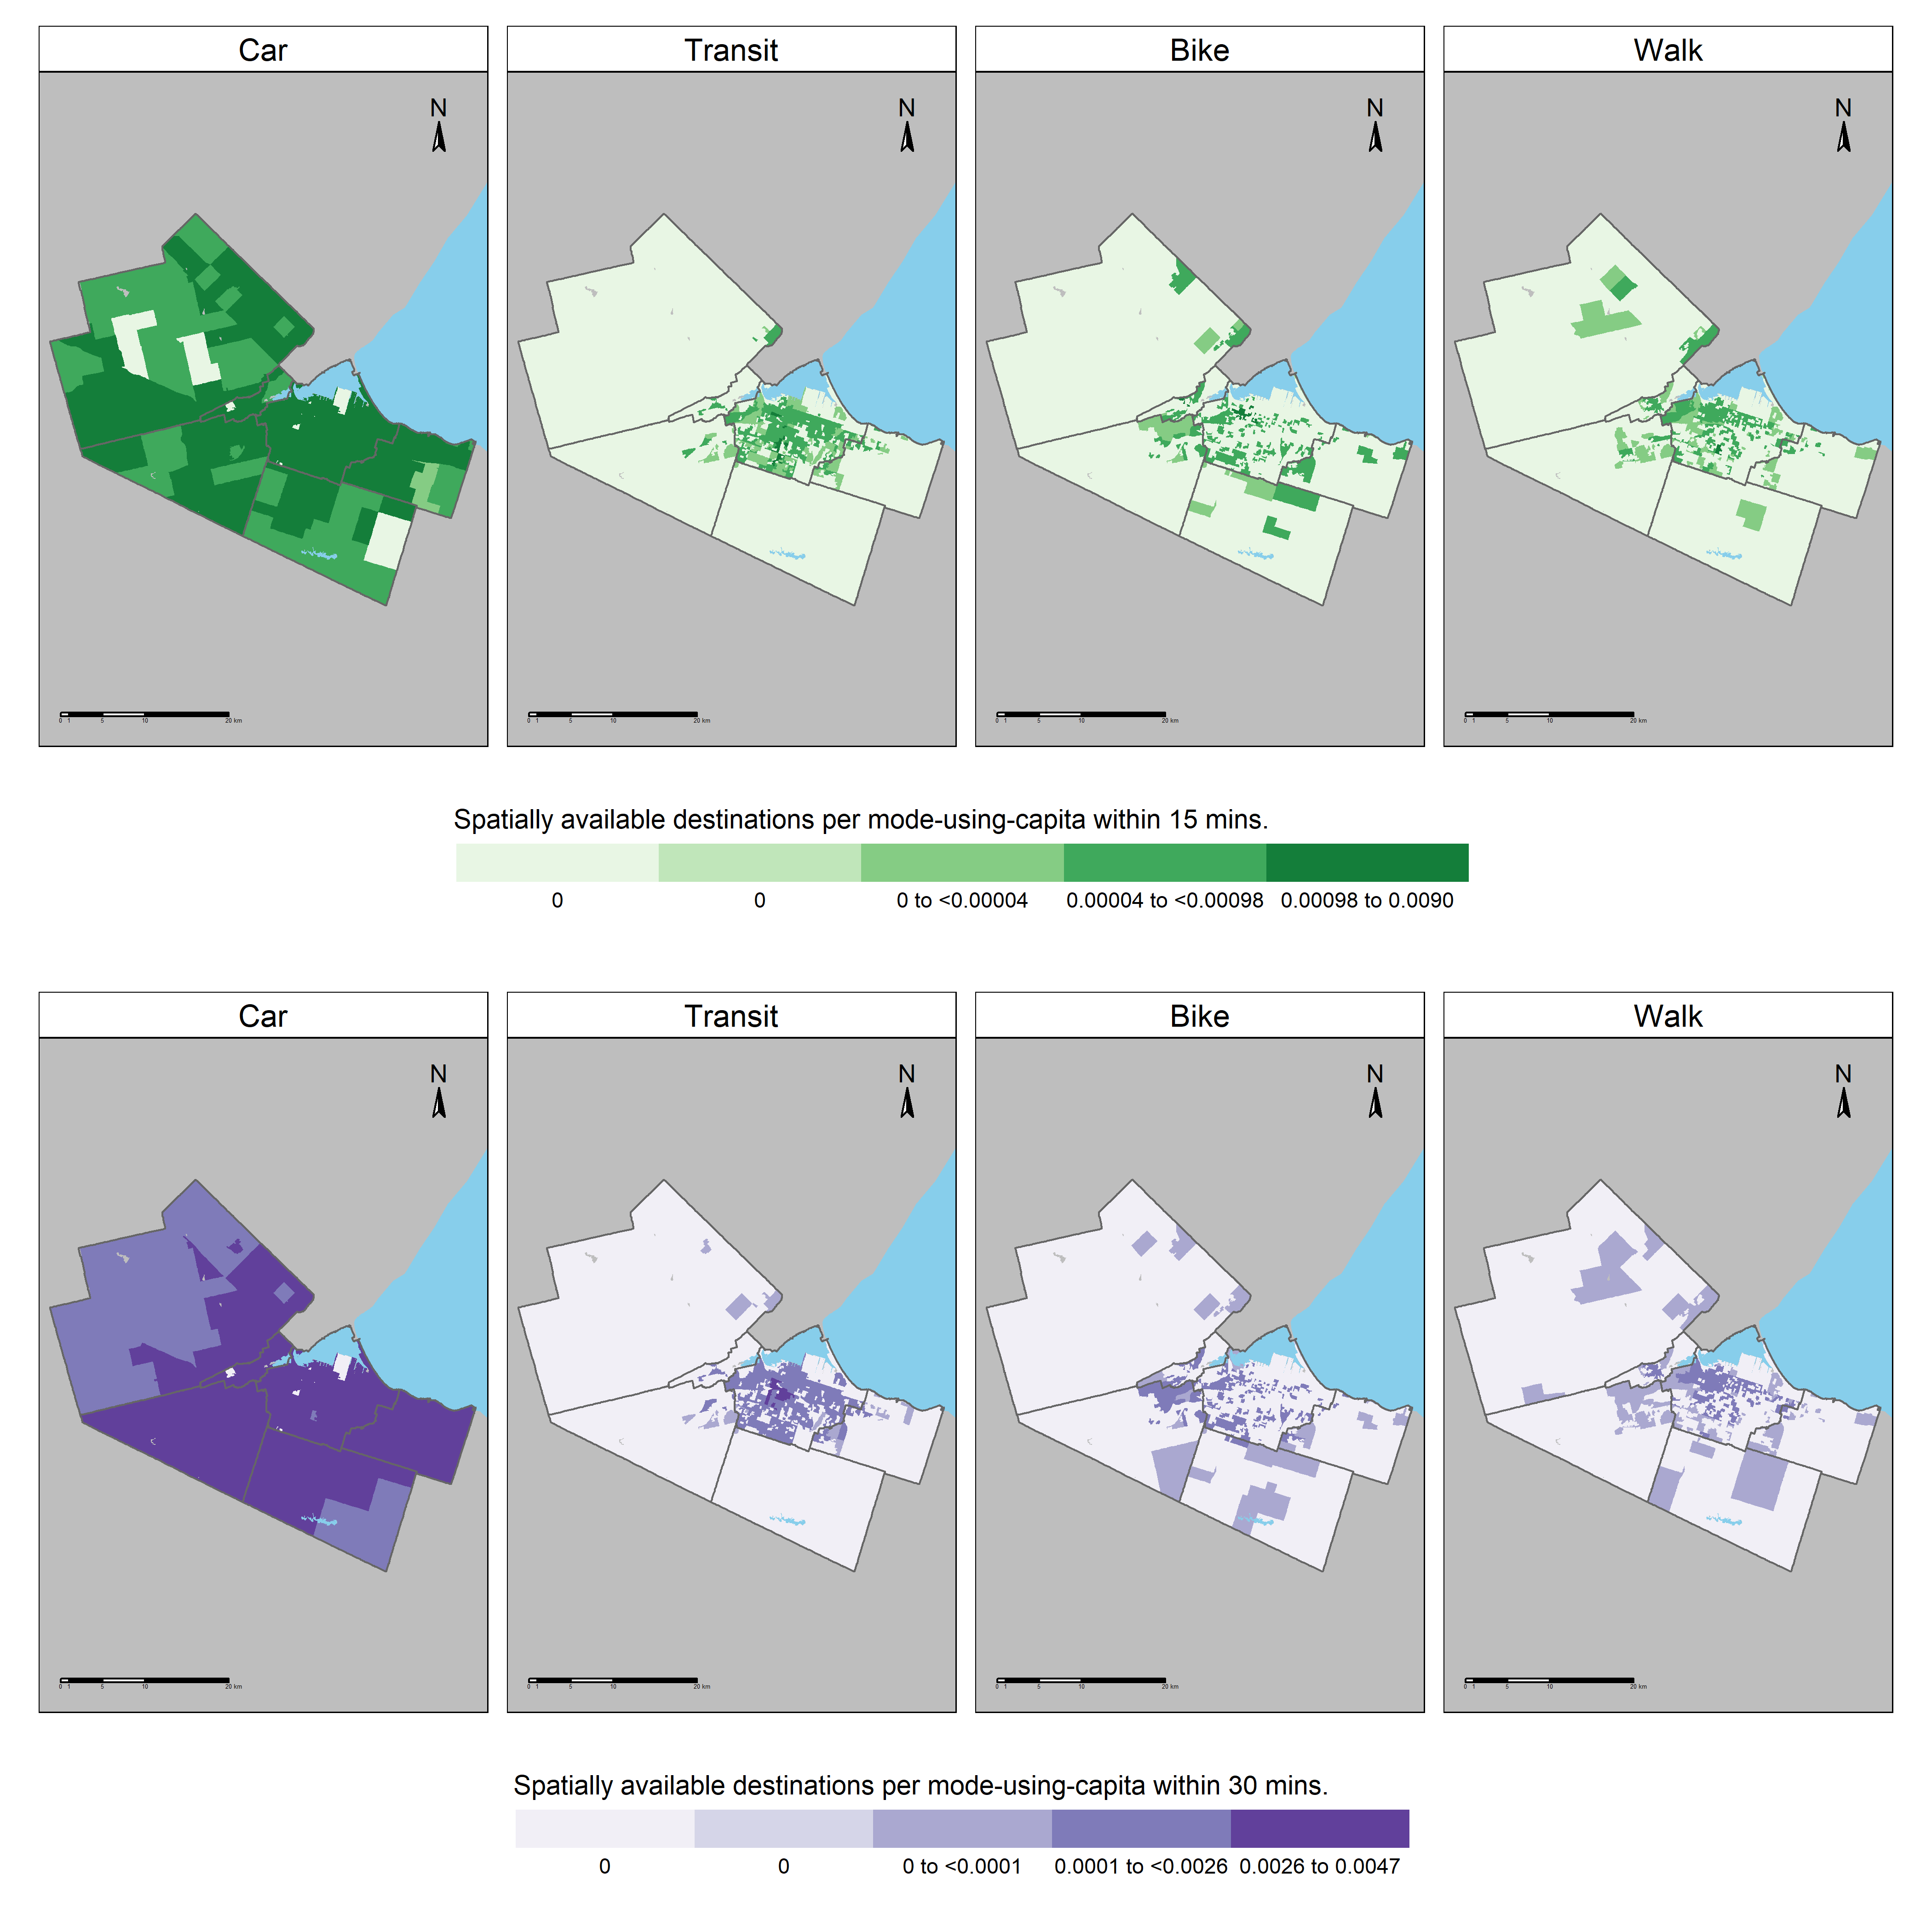
\includegraphics[width=6.25in,height=\textheight]{figures/Fig7-plot_Savail_smallv_measures.png}

}

\caption{\label{fig-Fig7}The spatial availability per mode-using-capita
measure. The number of care destinations that can be reached per
mode-using-capita, per DA, within 15 mins (top) and 30 mins (bottom).
Basemap shapefiles are retrieved from the 2021 Canadian census
\citep{governmentofcanadaCensusPopulation2023}, the Open Data Hamilton
Portal \citep{opendatahamiltonCityBoundary2023} and the USGS
\citep{greatlakesUSGS2010}.}

\end{figure}

Equity consideration and the consideration of travel time cut-off. We
can see signficant difference in the correlation between LICO-AT in a DA
and the modal per-capita spatial availability depending on if the 15
minute or 30 minute cut-off is considered. We can see 30 minute cut-off
is more generous, especially for the motorists that can almost reach all
destinations. As such, there is a weak positive correlation between for
motorists (0.1583927) and cyclists (0.2288479). However, there is
stronger positive correlation for those who walk (0.5715248) and use
transit (0.4185431). This is in line with literature XX. Areas that are
LICO-AT are clustered in higher density DAs in Hamilton-Centre, where
unconstrained and constrained access by all modes is high but access is
also high (or alright) for car and cycling in areas outside
Hamilton-Centre (areas with lower LICO-AT).

However, relationships are different assuming a 15 minute cut-off; all
modes see a weak but positive linear relationship between LICO-AT and
per-capita modal spatial availability however trends are reversed.
Cyclists and motorists now see a stronger relationship (cycle: 0.264636
and motorists: 0.4409378) than those who walk and use transit (walk:
0.1865794 and transit: 0.1262046). As mentioned, availability is high
for all modes in Hamilton-Centre where there is high LICO-AT, but
especially for faster modes like car and cycling. However, access for
all modes is not high outside of Hamilton-Centre. Because Car and
cycling does not have such an exceptional advantage in the rural
communities consider a 15-minute cut-off, the reverse trend emerges
where LICO-AT is correlated more strongly with cyclist and motorist
availability. This reversal in trend highlights the importance in
threshold selection as accessibility results are highly sensitive to the
assumptions of travel to destinations. Echos trends in literature X.
Empirical data is needed, but there is a bias in excluding
considerations for care destinations in conventional survey methods XX.

Overall, between the 15-minute and 30-minute cut-offs, there is a
positive relationship in per-capita availability and LICO-AT as well as
cumulative opportunity and LICO-AT. We know car mode provides
unconstrained and constrained access to opportunities; those who have a
car are covered. But we must plan for cities that are not reliant on
cars. Cycling has potential, but mostly in areas with low LICO-AT and
with the consideration for some risky cycling (level 1 and 2). Further,
comparing access to what cars can reach may not be the best approach --
most opportunities in the city of \textasciitilde500,000 can be reached
within 30-minutes. Is that necessary? Should that be the goal for all
modes? Or shall access by car be reduced while access by other modes
increased such that availability matches the proportion of the
mode-using population. Spatial availability can be used to consider
these options.

\hypertarget{discussion-and-conclusion}{%
\section{DISCUSSION AND CONCLUSION}\label{discussion-and-conclusion}}

This paper is first to conduct an exploratory feminist accessibility
analysis of care destinations -- one that counters the current
literature's emphasis on employment-related travel, a travel more
significant for men, and especially wealthy and educated men
\citep{robinlawWomenTransportNew1999, hansonGenderMobilityNew2010}. Its
aim is to challenge assumptions often made in transport planning tools
(i.e., that work is the most important place to access), and to provide
a tangible example of how one could gender-mainstream accessibility
analyses.

This study also contributes to the literature on sustainable travel
behaviour. Results indicate that care is most easily accessed in
Hamilton by car, an unsurprising result given its car-oriented design.
Previous research has found that mobility of care are more frequently
completed by car or by foot than by transit or by bicycle
\citep{ravensbergenExploratoryAnalysisMobility2022}. It is possible that
the car's ability to provide higher access to care destinations, as
observed in this study, shapes this tendency to complete care trips by
car. Then again, car use may be more frequent for care trips because
these trips tend to involve carrying things (e.g., groceries) or people
(e.g., children). Indeed, past qualitative work has found that many
prefer travelling by car for this type of trip due to convenience and
increased safety
\citep{maciejewskaHaveChildrenThus2019, carverParentalChauffeursWhat2013}.
Then again, care trips tend to be shorter than other trips
\citep{ravensbergenExploratoryAnalysisMobility2022}, making them ideal
for more sustainable travel modes, such as active modes (walking,
cycling) and public transport. The low access to care by foot identified
in this study is discouraging, given both people's tendency to use this
mode for care trips \citep{ravensbergenExploratoryAnalysisMobility2022},
and the benefits of walking as a travel mode, both for individuals,
cities, and the environment. Somewhat unexpectedly, access to care was
found to be low by transit and by foot and relatively high by bicycle.
Given that low income women, in particular, seem to be transit reliant
for care trips \citep{ravensbergenExploratoryAnalysisMobility2022}, this
result highlights both a potential bias against care trips by transit
and the equity implications of that bias. Though past work has found
that many barriers exist for cycling for care
\citep{ravensbergenVelomobilitiesCareLowcycling2020, ravensbergenFeministGeographiesCycling2019, sersliRidingAloneTogether2020},
the results of this study highlight the great potential of the bicycle
for easily accessing care.

The preliminary nature of this research also comes with its limitations
as a result of data availability. Firstly, the travel time estimations
assume free-flow network conditions: this may not drastically impact
walking travel time accuracy, but could impact car, transit and cycling
estimations. Secondly, the geometric centroids of DAs (origins) and
destinations (all care destinations) were used as inputs for travel time
calculations. DAs are created for the purpose of the census: they vary
in area and centroids may not necessarily align with where that
population may be beginning their journey to care destinations. Thirdly,
the cumulative opportunity accessibility measure is unconstrained and
does not consider competition. It is the sum of every care destination
that can be possibly reached, not taking into consideration the density
of neighbouring population that may also be reaching those destinations.
Fourthly, quality of the care destinations was not considered (e.g.,
access to a park is equal to access to a school). These limitations all
contribute to how accurately results reflect the quantitative access to
care landscape within Hamilton.

Future work on the accessibility of care will consider competition
factors through different accessibility measures, a higher spatial level
of travel time estimation, and the incorporation of different weightings
of care destination categories. In addition, future work will compare
care accessibility to work accessibility in Hamilton to highlight the
bias in planning towards jobs as well as substantive equity critiques.

\hypertarget{acknowledgements}{%
\section{ACKNOWLEDGEMENTS}\label{acknowledgements}}

This research was funded by the McMaster Undergraduate Student Research
Assistantship program of the Faculty of Social Sciences.

\hypertarget{author-contributions}{%
\section{AUTHOR CONTRIBUTIONS}\label{author-contributions}}

The authors confirm contribution to the paper as follows: study
conception and design: NM, LR, AS.; data collection: NM, AS; analysis
and interpretation of results: NM, AS, LR; draft manuscript preparation:
NM, LR, AS. All authors reviewed the results and approved the final
version of the manuscript.

\hypertarget{references}{%
\section*{References}\label{references}}
\addcontentsline{toc}{section}{References}

\hypertarget{appendix}{%
\section{Appendix}\label{appendix}}


  \bibliography{bibliography.bib}


\end{document}
